\documentclass[table]{beamer}
\usepackage{beamerthemesplit}
\usetheme{boxes}
\usecolortheme{seahorse}
% \useinnertheme{myboxes}
% \usepackage{amsmath}
% \usepackage[fleqn]{amsmath}
\usepackage{ifthen}
\usepackage{xspace}
\usepackage{multirow}
\usepackage{booktabs}
\usepackage{xcolor}
\usepackage[style=nature]{biblatex}
\newrobustcmd*{\footlessfullcite}{\AtNextCite{\renewbibmacro{title}{}\renewbibmacro{in:}{}}\footfullcite}
\AtEveryBibitem{\clearfield{month}}
\AtEveryCitekey{\clearfield{month}}

\usepackage{hyperref}
\hypersetup{pdfborder={0 0 0}, colorlinks=true, urlcolor=blue, linkcolor=blue, citecolor=blue}

% \usepackage[format=plain, labelsep=period, justification=raggedright, singlelinecheck=true, skip=2pt, font=sf]{caption}
\usepackage{caption}
\captionsetup[figure]{font=scriptsize, labelformat=empty, textformat=simple, justification=centering, skip=2pt}

% Make all footnotes smaller
\renewcommand{\footnotesize}{\scriptsize}

\definecolor{myGray}{gray}{0.9}
\colorlet{rowred}{red!30!white}

\setbeamertemplate{blocks}[rounded][shadow=true]

\setbeamercolor{defaultcolor}{bg=structure!30!normal text.bg,fg=black}
\setbeamercolor{block body}{bg=structure!30!normal text.bg,fg=black}
\setbeamercolor{block title}{bg=structure!50!normal text.bg,fg=black}

\newenvironment<>{varblock}[2][\textwidth]{%
  \setlength{\textwidth}{#1}
  \begin{actionenv}#3%
    \def\insertblocktitle{#2}%
    \par%
    \usebeamertemplate{block begin}}
  {\par%
    \usebeamertemplate{block end}%
  \end{actionenv}}

\newenvironment{displaybox}[1][\textwidth]
{
    \centerline\bgroup\hfill
    \begin{beamerboxesrounded}[lower=defaultcolor,shadow=true,width=#1]{}
}
{
    \end{beamerboxesrounded}\hfill\egroup
}

\newenvironment{onlinebox}[1][4cm]
{
    \newbox\mybox
    \newdimen\myboxht
    \setbox\mybox\hbox\bgroup%
        \begin{beamerboxesrounded}[lower=defaultcolor,shadow=true,width=#1]{}
    \centering
}
{
    \end{beamerboxesrounded}\egroup
    \myboxht\ht\mybox
    \raisebox{-0.25\myboxht}{\usebox\mybox}\hspace{2pt}
}

\newenvironment{mydescription}{
    \begin{description}
        \setlength{\leftskip}{-1.5cm}}
    {\end{description}}

\newenvironment{myitemize}{
    \begin{itemize}
        \setlength{\leftskip}{-.3cm}}
    {\end{itemize}}

% define formatting for footer
\newcommand{\myfootline}{%
    {\it
    \insertshorttitle
    \hspace*{\fill} 
    \insertshortauthor, \insertshortinstitute
    % \ifx\insertsubtitle\@empty\else, \insertshortsubtitle\fi
    \hspace*{\fill}
    \insertframenumber/\inserttotalframenumber}}

% set up footer
\setbeamertemplate{footline}{%
    \usebeamerfont{structure}
    \begin{beamercolorbox}[wd=\paperwidth,ht=2.25ex,dp=1ex]{frametitle}%
        \Tiny\hspace*{4mm}\myfootline\hspace{4mm}
    \end{beamercolorbox}}

% remove navigation bar
\beamertemplatenavigationsymbolsempty


% \newcommand{\change}[1]{{\color{blue} #1}\xspace}
\newcommand{\change}[1]{{\color{black} #1}\xspace}

\makeatletter
\newcommand*{\rom}[1]{\expandafter\@slowromancap\romannumeral #1@}
\makeatother

\newcommand{\myHangIndent}{\hangindent=5mm}

\newcommand{\citationNeeded}{\textcolor{magenta}{\textbf{[CITATION NEEDED!]}}\xspace}
\newcommand{\tableNeeded}{\textcolor{magenta}{\textbf{[TABLE NEEDED!]}}\xspace}
\newcommand{\figureNeeded}{\textcolor{magenta}{\textbf{[FIGURE NEEDED!]}}\xspace}
\newcommand{\highLight}[1]{\textcolor{magenta}{\MakeUppercase{#1}}}

\newcommand{\editorialNote}[1]{\textcolor{red}{[\textit{#1}]}}
\newcommand{\ignore}[1]{}
\newcommand{\addTail}[1]{\textit{#1}.---}
\newcommand{\super}[1]{\ensuremath{^{\textrm{#1}}}}
\newcommand{\sub}[1]{\ensuremath{_{\textrm{#1}}}}
\newcommand{\dC}{\ensuremath{^\circ{\textrm{C}}}}
\newcommand{\tb}{\hspace{2em}}

\providecommand{\e}[1]{\ensuremath{\times 10^{#1}}}

\newcommand{\mthnote}[2]{{\color{red} #2}\xspace}
\newcommand{\cwlnote}[2]{{\color{orange} #2}\xspace}

\newcommand{\ifTwoArgs}[3]{\ifthenelse{\equal{#1}{}\or\equal{#2}{}}{}{#3}\xspace}
\newcommand{\ifArg}[2]{\ifthenelse{\equal{#1}{}}{}{#2}\xspace}

\newcommand{\divTime}[1]{\ensuremath{\tau_{#1}}\xspace}
\newcommand{\divTimeVector}{\ensuremath{\boldsymbol{\divTime{}}}\xspace}
\newcommand{\divTimeIndex}[1]{\ensuremath{t_{#1}}\xspace}
\newcommand{\divTimeIndexVector}{\ensuremath{\mathbf{\divTimeIndex{}}}\xspace}
\newcommand{\divTimeMap}[1]{\ensuremath{T_{#1}}\xspace}
\newcommand{\divTimeMapVector}{\ensuremath{\mathbf{\divTimeMap{}}}\xspace}
\newcommand{\divTimeScaled}[2]{\ensuremath{\mathcal{T}_{#1\protect\ifTwoArgs{#1}{#2}{,}#2}}\xspace}
\newcommand{\divTimeScaledVector}{\ensuremath{\mathbf{\divTimeScaled{}{}}}\xspace}
\newcommand{\divTimeMean}{\ensuremath{\bar{\divTimeMap{}}}\xspace}
\newcommand{\divTimeVar}{\ensuremath{s^{2}_{\divTimeMap{}}}\xspace}
\newcommand{\divTimeDispersion}{\ensuremath{D_{\divTimeMap{}}}\xspace}
\newcommand{\divTimeNum}{\ensuremath{\lvert \divTimeVector \rvert}\xspace}
\newcommand{\demographicParams}[1]{\ensuremath{\Theta_{#1}}\xspace}
\newcommand{\demographicParamVector}{\ensuremath{\mathbf{\demographicParams{}}}\xspace}
\newcommand{\popSampleSize}[2]{\ensuremath{n_{#1\protect\ifTwoArgs{#1}{#2}{,}#2}}}
\newcommand{\gammaShape}[1]{\ensuremath{a_{#1}}\xspace}
\newcommand{\gammaScale}[1]{\ensuremath{b_{#1}}\xspace}
\newcommand{\betaA}[1]{\ensuremath{a_{#1}}\xspace}
\newcommand{\betaB}[1]{\ensuremath{b_{#1}}\xspace}
\newcommand{\integerPartitionSet}[1]{\ensuremath{a({#1})}\xspace}
\newcommand{\integerPartitionNum}[1]{\ensuremath{\lvert \integerPartitionSet{#1} \rvert}\xspace}
\newcommand{\concentrationParam}{\ensuremath{\chi}\xspace}
\newcommand{\stirlingFirst}[2]{\ensuremath{c(#1, #2)}\xspace}
\newcommand{\descendantThetaMean}[1]{\ensuremath{\bar{\theta}_{D\protect\ifArg{#1}{,}#1}}\xspace}
\newcommand{\numPriorSamples}{\ensuremath{\mathbf{n}}\xspace}
\newcommand{\paramSampleVector}[1]{\ensuremath{\Lambda_{#1}}\xspace}
\newcommand{\paramSampleMatrix}{\ensuremath{\boldsymbol{\paramSampleVector{}}}\xspace}
\newcommand{\ordered}{\ensuremath{\circ}\xspace}
\newcommand{\modelDPP}{\ensuremath{M_{DPP}}\xspace}
\newcommand{\modelDPPOrdered}{\ensuremath{M^{\ordered}_{DPP}}\xspace}
\newcommand{\modelUniform}{\ensuremath{M_{Uniform}}\xspace}
\newcommand{\modelUshaped}{\ensuremath{M_{Ushaped}}\xspace}
\newcommand{\modelOld}{\ensuremath{M_{msBayes}}\xspace}
\newcommand{\priorDPP}[1]{\ensuremath{DP(\concentrationParam #1)}\xspace}
\newcommand{\priorUniform}{\ensuremath{DU\{\integerPartitionSet{\npairs{}}\}}\xspace}
\newcommand{\priorOld}{\ensuremath{DU\{1, \ldots, \npairs{}\}}\xspace}
\newcommand{\powerSeriesOld}{\ensuremath{\mathcal{M}_{msBayes}}\xspace}
\newcommand{\powerSeriesUniform}{\ensuremath{\mathcal{M}_{Uniform}}\xspace}
\newcommand{\powerSeriesExp}{\ensuremath{\mathcal{M}_{Exp}}\xspace}
\newcommand{\empModelOld}{\ensuremath{\mathbf{M}_{msBayes}}\xspace}
\newcommand{\empModelUniform}{\ensuremath{\mathbf{M}_{Uniform}}\xspace}
\newcommand{\empModelDPP}{\ensuremath{\mathbf{M}_{DPP}}\xspace}
\newcommand{\empModelDPPInform}{\ensuremath{\mathbf{M}^{inform}_{DPP}}\xspace}
\newcommand{\empModelDPPSimple}{\ensuremath{\mathbf{M}^{simple}_{DPP}}\xspace}
\newcommand{\npModelDPP}{\ensuremath{\mathbb{M}_{DPP}}\xspace}
\newcommand{\npModelDPPOrdered}{\ensuremath{\mathbb{M}^{\ordered}_{DPP}}\xspace}


\bibliography{../bib/references}

\title[History of Lineages]{History of Lineages}
\subtitle{Chapter 11}

\author[J.\ Oaks]{
    Jamie Oaks\inst{1}
}
\institute[University of Washington]{
    \inst{1}%
        Kincaid Hall 524 \hspace{1em} \href{mailto:joaks1@gmail.com}{\texttt{joaks1@gmail.com}}
}

% \date{\today}
\date{April 11, 2014}

\begin{document}

% \maketitle
\begin{frame}
    \begin{columns}[c]
        \column{.5\textwidth}
            \maketitle
        \column{.5\textwidth}
            \begin{figure}
                \begin{center}
                \includegraphics[width=\textwidth]{../images/darwin-tol-copyright-boris-kulikov-2007.jpg}
                \caption{\tiny \copyright~2007 Boris Kulikov \href{http://boris-kulikov.blogspot.com/}{boris-kulikov.blogspot.com}}
                \end{center}
            \end{figure}
    \end{columns}
\end{frame}

\begin{frame}
    \frametitle{Acknowledgements}
    Some of the slides and images were stolen (with permission) from Dr. Mark Holder.
\end{frame}

\begin{frame}
\frametitle{Outline}
\tableofcontents
\end{frame}

%%%%%%%%%%%%%%%%%%%%%%%%%%%%%%%%%%%%%%%%%
\section{What is phylogenetics?}
%%%%%%%%%%%%%%%%%%%%%%%%%%%%%%%%%%%%%%%%%
\begin{frame}
    \frametitle{What is phylogenetics?}
    \begin{description}
        \item[Systematics] The science devoted to the study of the diversity of
            organisms, and the relationships among them.
        \item[Classification] The ordering of organisms into named groups on
            the basis of their relationships.
        \item[Phylogenetics] The science of inferring the genealogical
            relationships between species.
    \end{description}
\end{frame}

%%%%%%%%%%%%%%%%%%%%%%%%%%%%%%%%%%%%%%%%%
\section{Why is phylogenetics important?}
%%%%%%%%%%%%%%%%%%%%%%%%%%%%%%%%%%%%%%%%%

\begin{frame}
    \frametitle{Why is phylogenetics important?}
    \begin{quote}
    Seen in the light of evolution, biology is, perhaps, intellectually the
    most satisfying and inspiring science. Without that light it becomes a pile
    of sundry facts some of them interesting or curious but making no
    meaningful picture as a whole.
    \end{quote}

    \myHangIndent
    - Dobzhansky, T. (1973). Nothing in biology makes sense except in the light
    of evolution. The American Biology Teacher 35:125--129.

    \bigskip

    \begin{quote}
    \ldots nothing in evolution makes sense except in the light of phylogeny \ldots
    \end{quote}

    \myHangIndent
    - Society of Systematic Biologists
\end{frame}

\begin{frame}
    \frametitle{Why is phylogenetics important?}
    We cannot understand biodiversity without its blueprint: the tree of life.
    \begin{figure}
        \begin{center}
        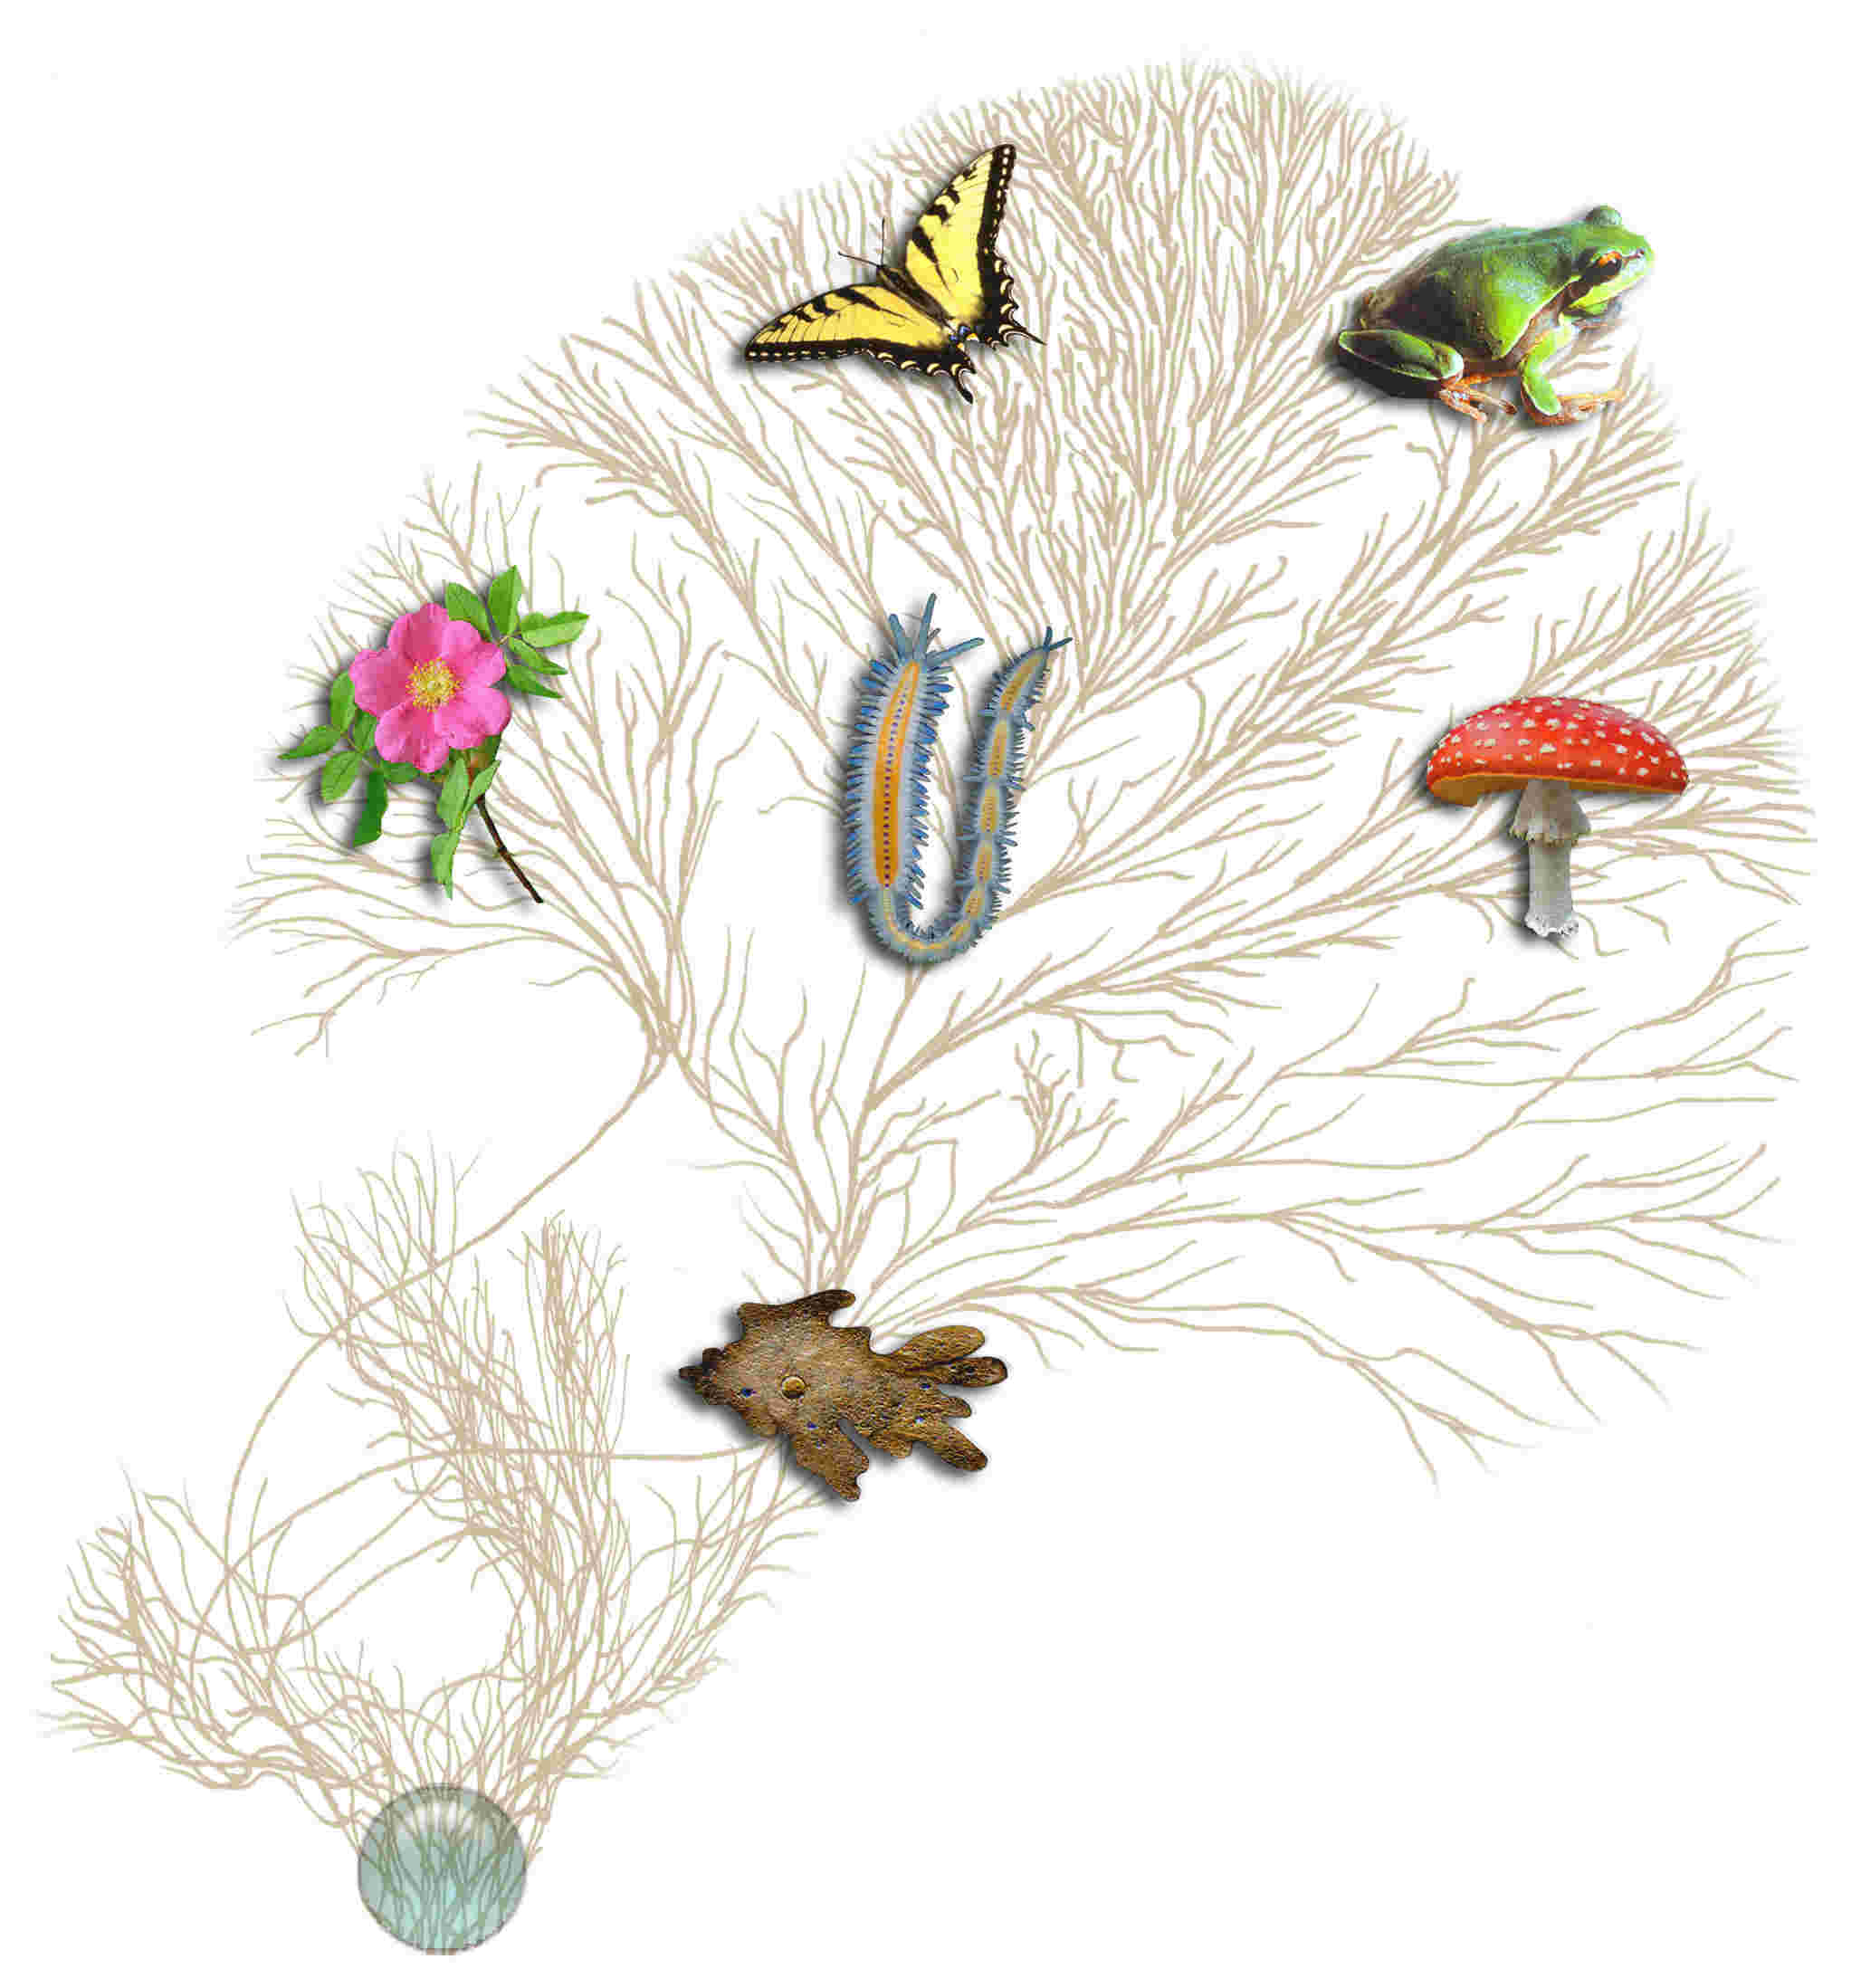
\includegraphics[width=0.55\textwidth]{../images/treeoflife.jpg}
        \caption{\tiny \copyright~2007 Tree of Life Web Project \href{http://tolweb.org/tree/}{tolweb.org}}
        \end{center}
    \end{figure}
\end{frame}

\begin{frame}
    \frametitle{Why is phylogenetics important?}
    \begin{columns}[c]
        \column{.5\textwidth}
        Bergmann's Rule
            \begin{onlyenv}<1->
                \begin{center}
                    \begin{tikzpicture}
                    [scale=0.35,auto=left,every node/.style={circle}]%,fill=blue!20}]
                        \draw [<->,thick] (0,10) -- (0,0) -- (14,0);
                        \node [label=below: {\sffamily Latitude}](xl) at (7.5,0.5) {};
                        \node [label=left: {\sffamily Mass}](yl) at (0,5) {};
                        \node [inode, label={[label distance=-5pt]0:\small\sffamily\bfseries A}](a) at (1,1) {};
                        \node [inode, label={[label distance=-5pt]0:\small\sffamily\bfseries B}](d) at (2.5,0.8) {};
                        \node [inode, label={[label distance=-5pt]0:\small\sffamily\bfseries C}](c) at (2,2.5) {};
                        \node [inode, color=blue, label={[label distance=-5pt]0:\small\sffamily\bfseries D}](e) at (7,7.5) {};
                        \node [inode, color=blue, label={[label distance=-5pt]0:\small\sffamily\bfseries E}](f) at (8.1,9.1) {};
                        \node [inode, color=blue, label={[label distance=-5pt]0:\small\sffamily\bfseries F}](b) at (10,10) {};
                    
                    \end{tikzpicture}
                \end{center}
            \end{onlyenv}
        \column{.5\textwidth}
            \begin{onlyenv}<2>
                \begin{center}
                    \begin{tikzpicture}
                    [scale=0.35,auto=left,every node/.style={circle}]%,fill=blue!20}]
                        \node [inode, color=black, label={[label distance=-5pt]90:\small\sffamily\bfseries A}](a) at (1, 7) {};
                        \node [inode, color=black, label={[label distance=-5pt]90:\small\sffamily\bfseries B}](b) at (3, 7) {};
                        \node [inode, color=black, label={[label distance=-5pt]90:\small\sffamily\bfseries C}](c) at (5, 7) {};
                        \node [inode, color=blue, label={[label distance=-5pt]90:\small\sffamily\bfseries D}](d) at (7, 7) {};
                        \node [inode, color=blue, label={[label distance=-5pt]90:\small\sffamily\bfseries E}](e) at (9, 7) {};
                        \node [inode, color=blue, label={[label distance=-5pt]90:\small\sffamily\bfseries F}](f) at (11, 7) {};
          
                        \draw [very thick] (a) -- (3,5) -- (4,6) -- (c);
                        \draw [very thick] (4,6) -- (3.5, 6.5);
                        \draw [very thick] (3.5, 6.5) -- (b);
                        \draw [very thick, draw=blue] (d) -- (9,5) -- (10,6) -- (f);
                        \draw [very thick, draw=blue] (10,6) -- (9.5, 6.5);
                        \draw [very thick, draw=blue] (9.5, 6.5) -- (e);
                        \draw [very thick] (3,5) -- (6,-4) -- (7.5, 0.5);
                        \draw [very thick, draw=blue] (7.5, 0.5) -- (9, 5);
                        \draw [very thick] (6,-4) -- (6, -5);
                    
                    \end{tikzpicture}
                \end{center}
            \end{onlyenv}

            \begin{onlyenv}<3>
                \begin{center}
                    \begin{tikzpicture}
                    [scale=0.35,auto=left,every node/.style={circle}]%,fill=blue!20}]
                        \node [inode, color=black, label={[label distance=-5pt]90:\small\sffamily\bfseries A}](a) at (1, 7) {};
                        \node [inode, color=blue, label={[label distance=-5pt]90:\small\sffamily\bfseries E}](b) at (3, 7) {};
                        \node [inode, color=black, label={[label distance=-5pt]90:\small\sffamily\bfseries C}](c) at (5, 7) {};
                        \node [inode, color=blue, label={[label distance=-5pt]90:\small\sffamily\bfseries D}](d) at (7, 7) {};
                        \node [inode, color=black, label={[label distance=-5pt]90:\small\sffamily\bfseries B}](e) at (9, 7) {};
                        \node [inode, color=blue, label={[label distance=-5pt]90:\small\sffamily\bfseries F}](f) at (11, 7) {};
          
                        \draw [very thick] (a) -- (3,5) -- (4,6) -- (c);
                        \draw [very thick] (4,6) -- (3.5, 6.5);
                        \draw [very thick, draw=blue] (3.5, 6.5) -- (b);
                        \draw [very thick, draw=blue] (d) -- (9,5) -- (10,6) -- (f);
                        \draw [very thick, draw=blue] (10,6) -- (9.5, 6.5);
                        \draw [very thick] (9.5, 6.5) -- (e);
                        \draw [very thick] (3,5) -- (6,-4) -- (7.5, 0.5);
                        \draw [very thick, draw=blue] (7.5, 0.5) -- (9, 5);
                        \draw [very thick] (6,-4) -- (6, -5);
                    
                    \end{tikzpicture}
                \end{center}
            \end{onlyenv}
    \end{columns}
\end{frame}

\begin{frame}
    \frametitle{Why is phylogenetics important?}
    \begin{itemize}
        \item Every field of biology studies organisms.
        \item These organisms are \textbf{not} independent.
        \item To analyze biological data correctly we need to account for
            shared history among organisms.
    \end{itemize}
\end{frame}

% Classification before phylogeny -- been classifying stuff since hg days -> tends to form hiearchies
% Linneaus formalized this
% Evolution gave the framework behind why hiearchies were intuitive

%%%%%%%%%%%%%%%%%%%%%%%%%%%%%%%%%%%%%%%%%%%%%%%%%%%
\section{Tree and character terminology and basics}
%%%%%%%%%%%%%%%%%%%%%%%%%%%%%%%%%%%%%%%%%%%%%%%%%%%

\begin{frame}
\frametitle{Outline}
\tableofcontents[currentsection]
\end{frame}

\begin{frame}
    \frametitle{Tree terminology}
    \begin{center}
        \begin{tikzpicture}
        [xscale=0.75,yscale=0.55,auto=left,every node/.style={circle}]%,fill=blue!20}]
            \node [inode, color=black, label={[label distance=-5pt]90:\small\sffamily\bfseries A}](a) at (1, 7) {};
            \node [inode, color=black, label={[label distance=-5pt]90:\small\sffamily\bfseries B}](b) at (3, 7) {};
            \node [inode, color=black, label={[label distance=-5pt]90:\small\sffamily\bfseries C}](c) at (5, 7) {};
            \node [inode, color=black, label={[label distance=-5pt]90:\small\sffamily\bfseries D}](d) at (7, 7) {};
            \node [inode, color=black, label={[label distance=-5pt]90:\small\sffamily\bfseries E}](e) at (9, 7) {};
            \node [inode, color=black, label={[label distance=-5pt]90:\small\sffamily\bfseries F}](f) at (11, 7) {};
            \node [inode](bc) at (4, 5)  {};
            \node [inode](ef) at (10, 5)  {};
            \node [inode](abc) at (3, 3)  {};
            \node [inode] (abcd) at (4, 1)  {};
            \node [inode](r) at (6, -3)  {};
          
            \foreach \from/\to in {bc/b,bc/c,abc/bc,abc/a,abcd/abc,abcd/d,r/abcd,r/ef,ef/e,ef/f}
                \draw [very thick] (\from) -- (\to);
            
            \draw [thick, <-] (2.9, 2.9) -- (2.4, 2.4) node[align=right, left] {\sffamily internal node};
            \draw [thick, <-] (8.1, 0.9) -- (8.6, 0.4) node[align=left, right] {\sffamily branch};
            \draw [thick, <-] (11.1, 6.9) -- (11.6, 6.4) node[align=left, right] {\sffamily terminal node \\(or leaf, tip)};
            \draw [thick, <-] (5.9, -3.1) -- (5.4, -3.6) node[align=right, left] {\sffamily root node};
        
        \end{tikzpicture}
    \end{center}
\end{frame}

\begin{frame}
    \frametitle{Tree terminology}
    \begin{description}
        \item[Terminal nodes]
            Also called ``leaves'', ``tips,'' or ``taxa.''
            These represent our observations (data).
            Depending on the study, this could be a species, population,
            individual organism, or a gene.
        \item[Internal nodes]
            These represent ancestors of leaves.
            These are typically not observed.
            Again, these could be an ancestral species, population,
            organism, gene, etc.
        \item[Root node]
            The most recent common ancestor (MRCA) of all the tips.  Sometimes
            the root node is not known or estimated, and so you will often see
            trees ``unrooted.''
        \item[Branches]
            These represent topology, or the relationships among the nodes.
            Sometimes the length of the branches represent the amount of
            evolutionary change or duration of time.
    \end{description}
\end{frame}

\begin{frame}
    \frametitle{Interpreting trees}
    \uncover<2->{These trees are the same! The proximity of the tips does not matter, you
    have to follow the branches to interpret the relationships.}
    \vspace{-1cm}
    \begin{columns}[c]
        \column{.5\textwidth}
        \begin{center}
            \begin{tikzpicture}
            [xscale=0.5,yscale=0.55,auto=left,every node/.style={circle}]%,fill=blue!20}]
              \node [inode, color=black, label={[label distance=-5pt]90:\small\sffamily\bfseries A}](a) at (1, 7) {};
              \node [inode, color=black, label={[label distance=-5pt]90:\small\sffamily\bfseries B}](b) at (3, 7) {};
              \node [inode, color=black, label={[label distance=-5pt]90:\small\sffamily\bfseries C}](c) at (5, 7) {};
              \node [inode, color=black, label={[label distance=-5pt]90:\small\sffamily\bfseries D}](d) at (7, 7) {};
              \node [inode, color=black, label={[label distance=-5pt]90:\small\sffamily\bfseries E}](e) at (9, 7) {};
              \node [inode, color=black, label={[label distance=-5pt]90:\small\sffamily\bfseries F}](f) at (11, 7) {};
              \node [inode](bc) at (4, 5)  {};
              \node [inode](ef) at (10, 5)  {};
              \node [inode](abc) at (3, 3)  {};
              \node [inode] (abcd) at (4, 1)  {};
              \node [inode](r) at (6, -3)  {};
            
              \foreach \from/\to in {bc/b,bc/c,abc/bc,abc/a,abcd/abc,abcd/d,r/abcd,r/ef,ef/e,ef/f}
                \draw [very thick] (\from) -- (\to);
              
            \end{tikzpicture}
        \end{center}
        \column{.5\textwidth}
        \begin{center}
            \begin{tikzpicture}
            [xscale=0.5,yscale=0.55,auto=left,every node/.style={circle}]%,fill=blue!20}]
                \node [inode, color=black, label={[label distance=-5pt]90:\small\sffamily\bfseries A}](a) at (7, 7) {};
                \node [inode, color=black, label={[label distance=-5pt]90:\small\sffamily\bfseries B}](b) at (3, 7) {};
                \node [inode, color=black, label={[label distance=-5pt]90:\small\sffamily\bfseries C}](c) at (5, 7) {};
                \node [inode, color=black, label={[label distance=-5pt]90:\small\sffamily\bfseries D}](d) at (1, 7) {};
                \node [inode, color=black, label={[label distance=-5pt]90:\small\sffamily\bfseries F}](e) at (9, 7) {};
                \node [inode, color=black, label={[label distance=-5pt]90:\small\sffamily\bfseries E}](f) at (11, 7) {};
                \node [inode](bc) at (4, 5)  {};
                \node [inode](ef) at (10, 5)  {};
                \node [inode](abc) at (5, 3)  {};
                \node [inode] (abcd) at (4, 1)  {};
                \node [inode](r) at (6, -3)  {};
              
                \foreach \from/\to in {bc/b,bc/c,abc/bc,abc/a,abcd/abc,abcd/d,r/abcd,r/ef,ef/e,ef/f}
                    \draw [very thick] (\from) -- (\to);
              
            \end{tikzpicture}
        \end{center}
    \end{columns}
\end{frame}


\begin{frame}
    \frametitle{Interpreting rooted vs unrooted trees}
    \uncover<2->{\raggedleft Where should the root go?}
    \vspace{-0.5cm}
    \begin{columns}[c]
        \column{.5\textwidth}
        \begin{center}
            \begin{tikzpicture}
            [xscale=0.4,yscale=0.55,auto=left,every node/.style={circle}]%,fill=blue!20}]
                \node [inode, color=black, label={[label distance=-5pt]90:\small\sffamily\bfseries A}](a) at (1, 7) {};
                \node [inode, color=black, label={[label distance=-5pt]90:\small\sffamily\bfseries B}](b) at (3, 7) {};
                \node [inode, color=black, label={[label distance=-5pt]90:\small\sffamily\bfseries C}](c) at (5, 7) {};
                \node [inode, color=black, label={[label distance=-5pt]90:\small\sffamily\bfseries D}](d) at (7, 7) {};
                \node [inode, color=black, label={[label distance=-5pt]90:\small\sffamily\bfseries E}](e) at (9, 7) {};
                \node [inode, color=black, label={[label distance=-5pt]90:\small\sffamily\bfseries F}](f) at (11, 7) {};
                \node [inode](bc) at (4, 5)  {};
                \node [inode](ef) at (10, 5)  {};
                \node [inode](abc) at (3, 3)  {};
                \node [inode] (abcd) at (4, 1)  {};
                \node [inode](r) at (6, -3)  {};
              
                \foreach \from/\to in {bc/b,bc/c,abc/bc,abc/a,abcd/abc,abcd/d,r/abcd,r/ef,ef/e,ef/f}
                    \draw [very thick] (\from) -- (\to);
              
            \end{tikzpicture}
        \end{center}
        \column{.5\textwidth}
        \begin{center}
            \begin{tikzpicture}
            [xscale=0.35, yscale=0.6, auto=left,every node/.style={circle}]%,fill=blue!20}]
                \node [tnode](d) at (1,10.5) {C};
                \node [tnode](a) at (3,11) {B};
                \node [tnode](c) at (3,6) {A};
                \node [tnode](e) at (13,10) {E};
                \node [tnode](f) at (16,7) {F};
                \node [tnode](b) at (14,2) {D};
                \node [inode](ef) at (13,9) {};
                \node [inode](efb) at (12, 8) {};
                \node [inode](adc) at (4,7) {};
                \node [inode](ad) at (2, 10) {};
              
                \foreach \from/\to in {efb/ef,efb/b,adc/c,adc/efb,ad/a,ad/d,ad/adc,ef/e,ef/f}
                    \draw [very thick] (\from) -- (\to);
                \uncover<3->{\draw [very thick, <-] (12.4, 8.6) -- (11.4, 9.6);}
            
            \end{tikzpicture}
        \end{center}
    \end{columns}
\end{frame}
                
\begin{frame}
    \frametitle{Tree branch lengths}
    \vspace{-0.25cm}
    \begin{description}
        \item[Cladogram] A phylogenetic tree where branches only depict
            relationships; branch \textbf{lengths} have no meaning.  Methods
            that produce cladograms usually estimate \textbf{unrooted} trees; the
            root is assumed or implied via an outgroup.
    \end{description}
    \begin{figure}
        \begin{center}
            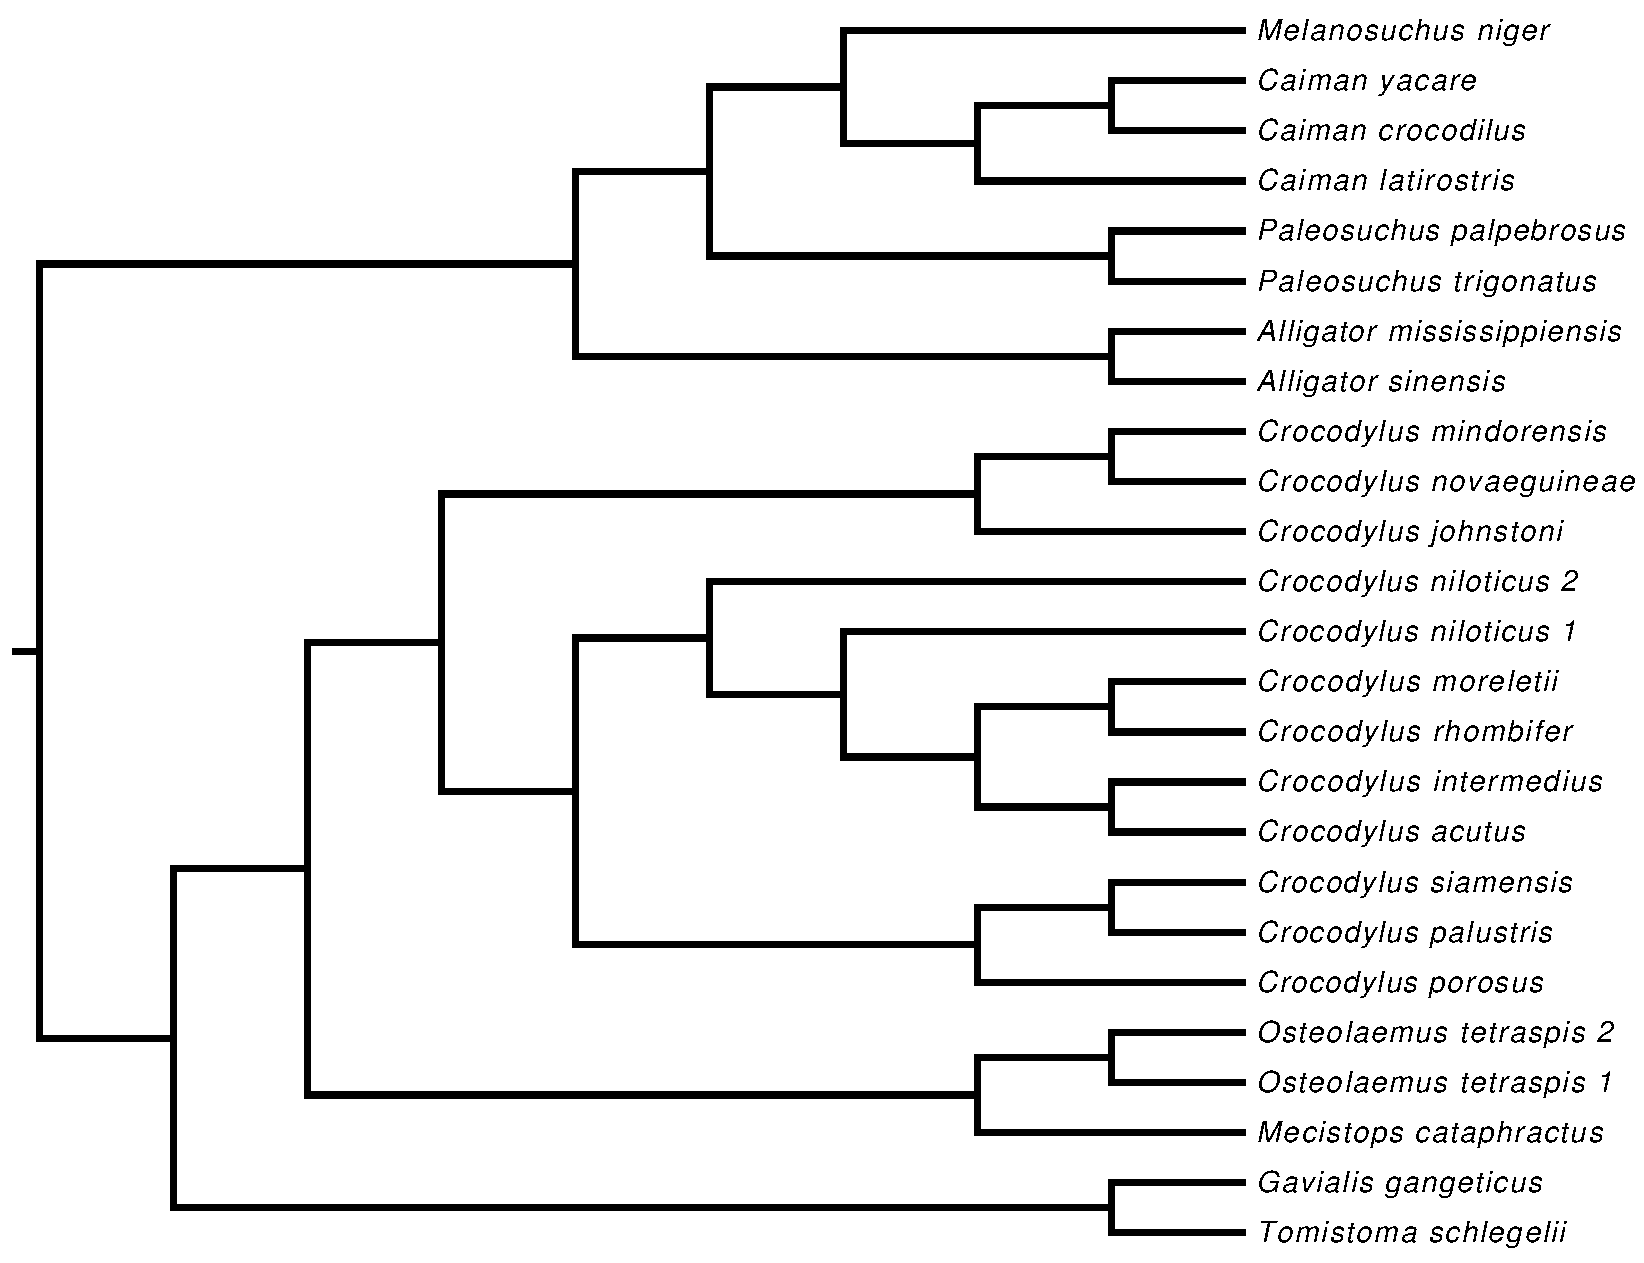
\includegraphics[width=0.65\textwidth]{../images/crocodylia-species-tree-cladogram.pdf}
        \end{center}
    \end{figure}
\end{frame}

\begin{frame}
    \frametitle{Tree branch lengths}
    \vspace{-0.25cm}
    \begin{description}
        \item[Phylogram] {\small A phylogenetic tree with branch lengths that are
            proportional to the amount of evolutionary change.  Methods that
            produce phylograms usually estimate \textbf{unrooted} trees; the
        root is assumed or implied via an outgroup.}
    \end{description}
    \begin{figure}
        \begin{center}
            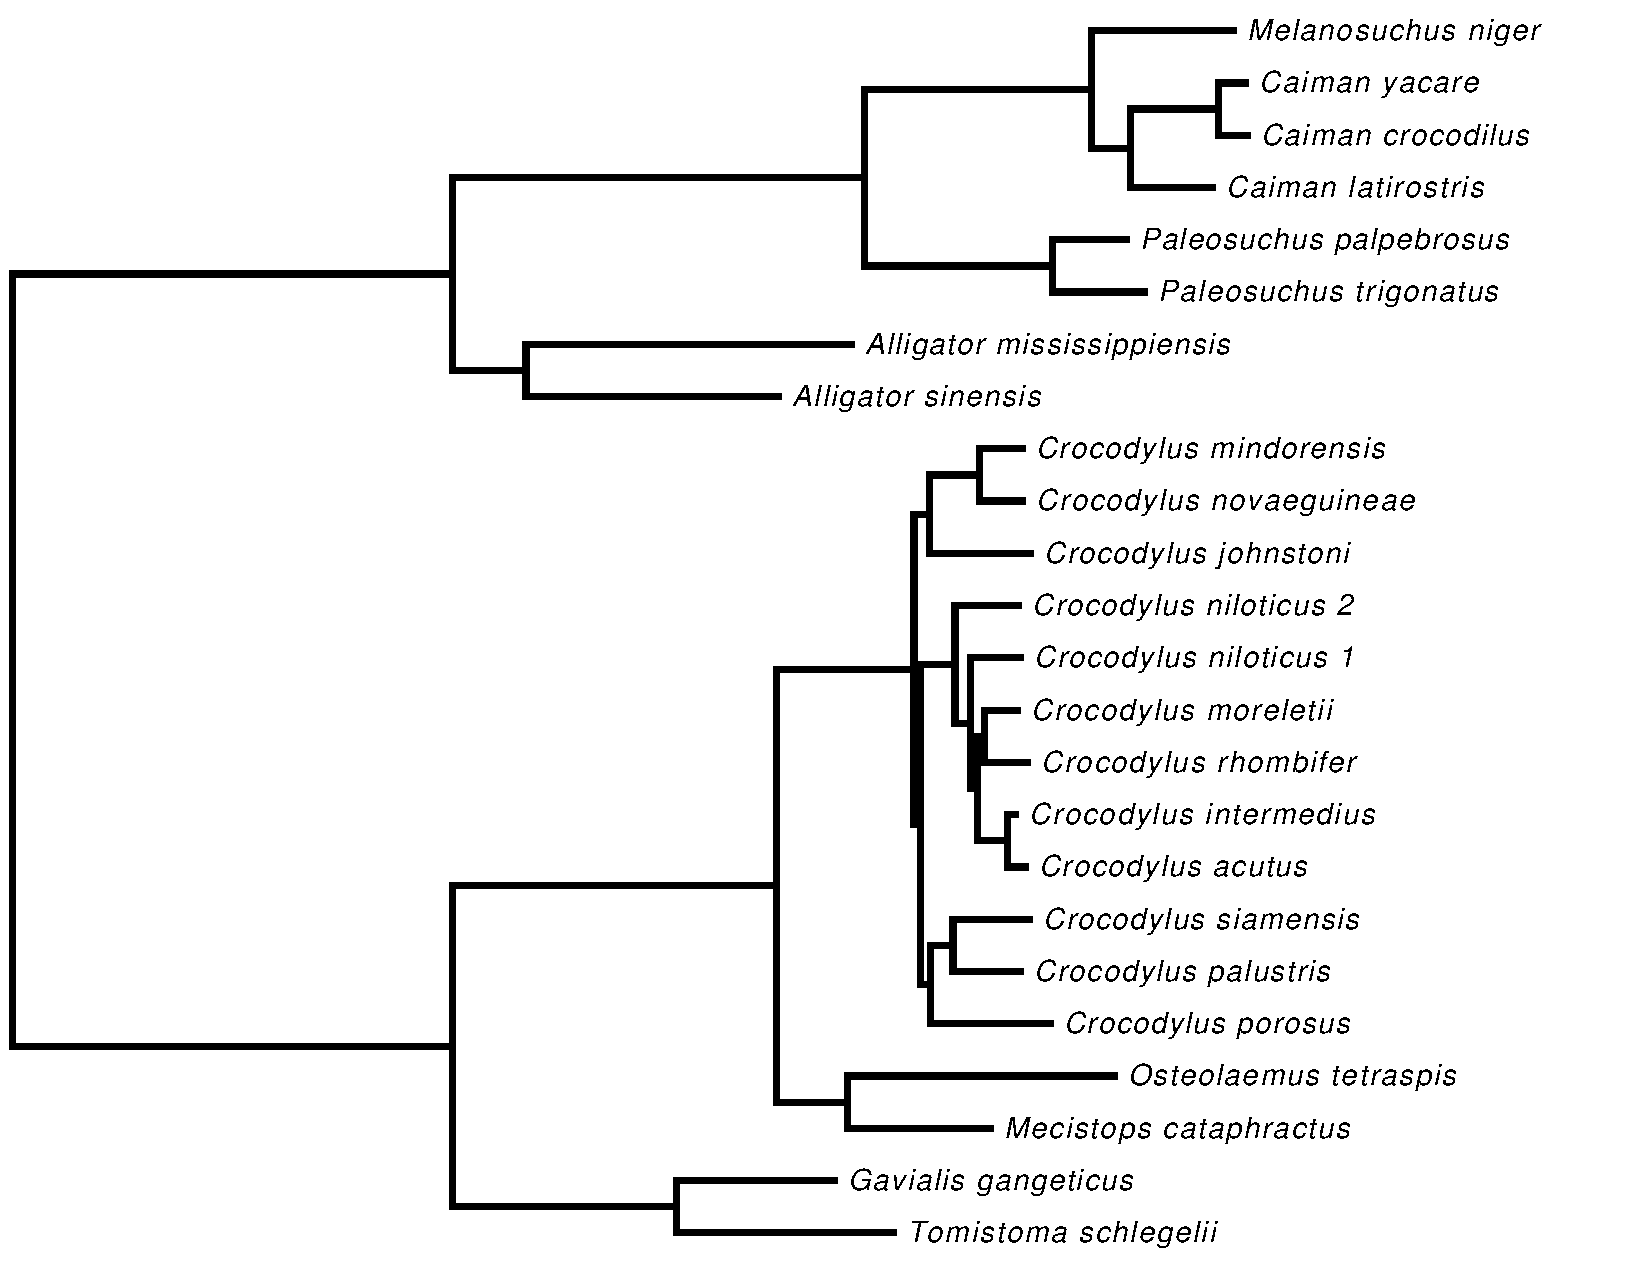
\includegraphics[width=0.65\textwidth]{../images/crocodylia-ml.pdf}
        \end{center}
    \end{figure}
\end{frame}

\begin{frame}
    \frametitle{Tree branch lengths}
    \vspace{-0.25cm}
    \begin{description}
        \item[Chronogram] A phylogenetic tree with branch lengths that are
            proportional to time duration. Methods that produce chronograms
            estimate \textbf{rooted} trees.
    \end{description}
    \begin{figure}
        \begin{center}
            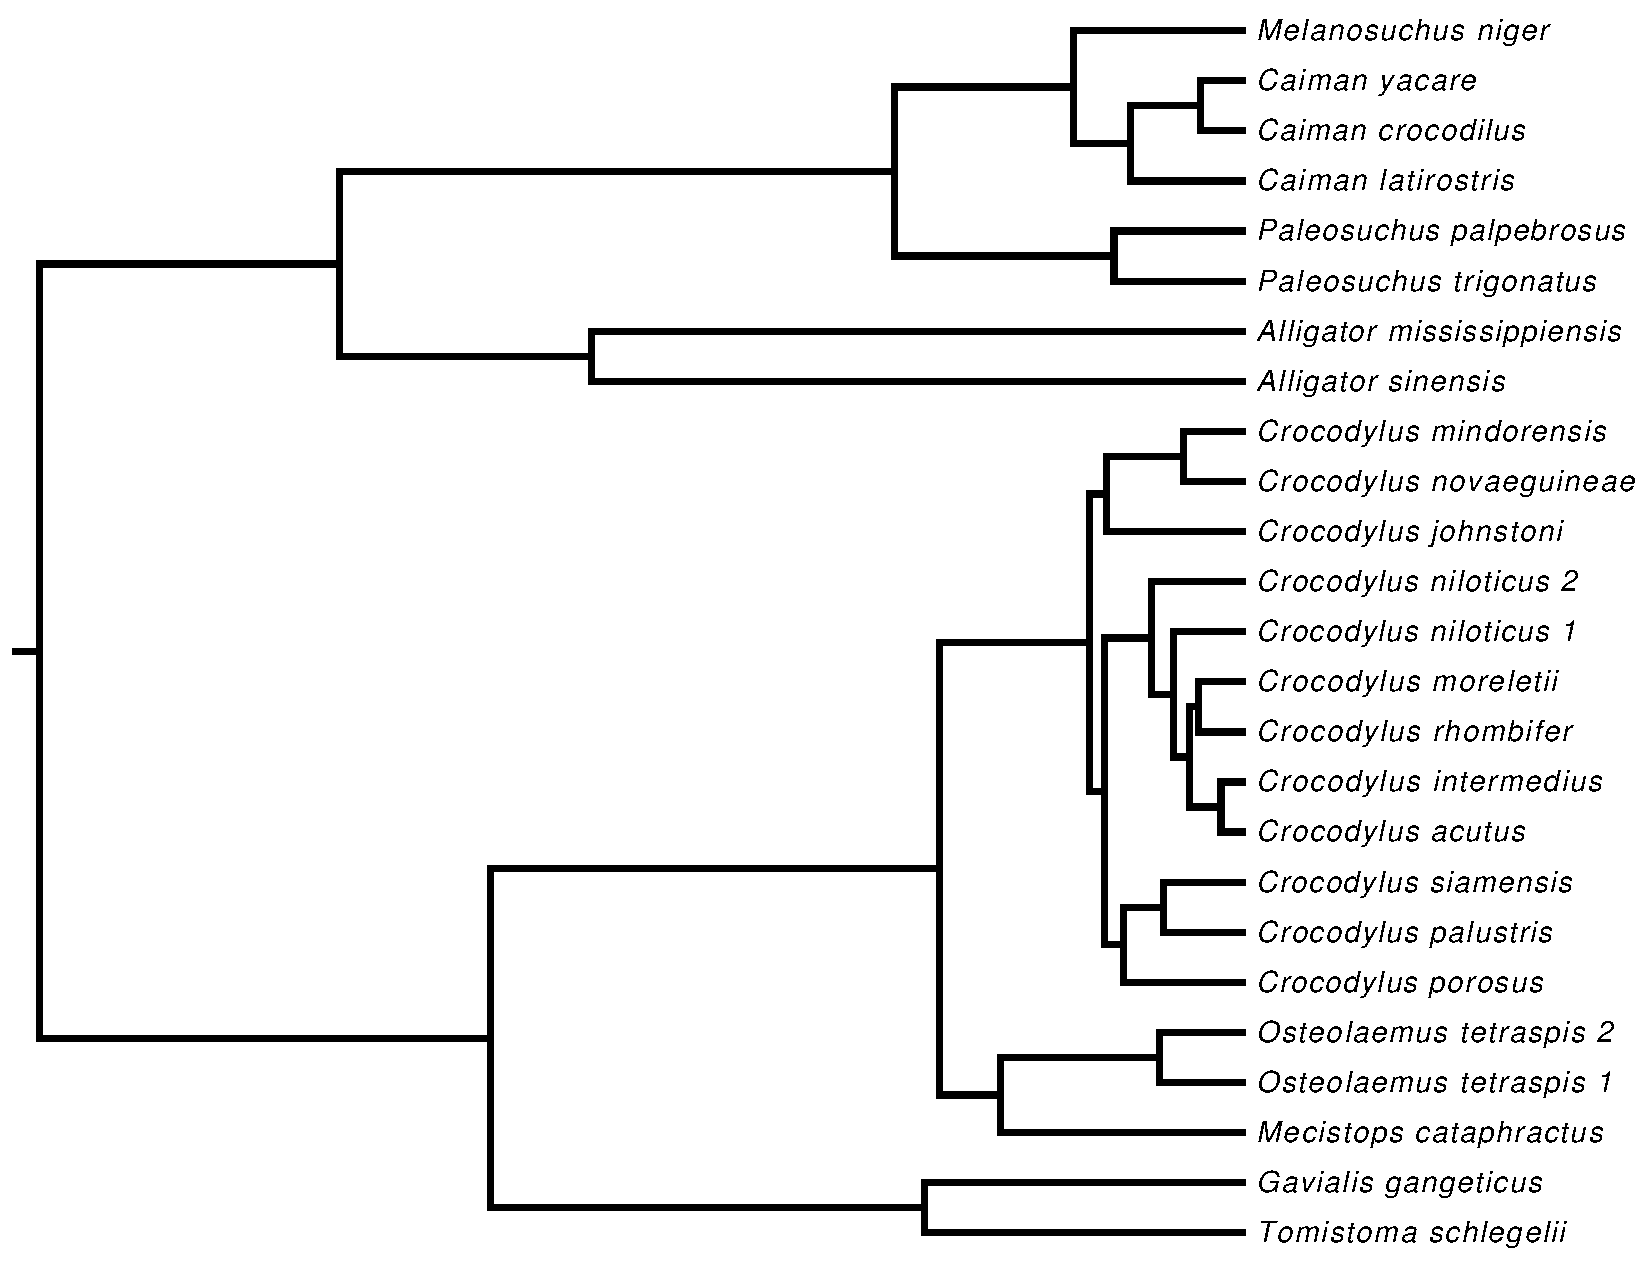
\includegraphics[width=0.7\textwidth]{../images/crocodylia-species-tree-square.pdf}
        \end{center}
    \end{figure}
\end{frame}

\begin{frame}
    \frametitle{Style of presentation varies a lot}
    \begin{center}
        \includegraphics<1>[width=0.8\textwidth]{../images/crocodylia-species-tree-square.pdf}
        \includegraphics<2>[width=0.8\textwidth]{../images/crocodylia-species-tree-round.pdf}
        \includegraphics<3>[width=0.8\textwidth]{../images/crocodylia-species-tree-triangle.pdf}
        \includegraphics<4>[width=0.8\textwidth]{../images/crocodylia-species-tree-circle.pdf}
    \end{center}
\end{frame}

\begin{frame}
    \frametitle{Classification: Grouping leaves---the good}
    \begin{description}
        \item[Monophyletic group] A group that consists of an ancestor and all
            of its descendants. Also called a clade or ``natural'' group. The
            basis of phylogenetic classification. Good!
    \end{description}
    \vspace{-0.45cm}
    \begin{center}
        \begin{onlyenv}<1>
        \begin{tikzpicture}
        [xscale=0.75,yscale=0.55,auto=left,every node/.style={circle}]%,fill=blue!20}]
            \node [inode, color=green, label={[label distance=-5pt]90:\sffamily\bfseries \textcolor{green}{A}}](a) at (1, 7) {};
            \node [inode, color=green, label={[label distance=-5pt]90:\sffamily\bfseries \textcolor{green}{B}}](b) at (3, 7) {};
            \node [inode, color=green, label={[label distance=-5pt]90:\sffamily\bfseries \textcolor{green}{C}}](c) at (5, 7) {};
            \node [inode, color=black, label={[label distance=-5pt]90:\sffamily\bfseries D}](d) at (7, 7) {};
            \node [inode, color=black, label={[label distance=-5pt]90:\sffamily\bfseries E}](e) at (9, 7) {};
            \node [inode, color=black, label={[label distance=-5pt]90:\sffamily\bfseries F}](f) at (11, 7) {};
            \node [inode, color=green](bc) at (4, 5)  {};
            \node [inode](ef) at (10, 5)  {};
            \node [inode, color=green](abc) at (3, 3)  {};
            \node [inode] (abcd) at (4, 1)  {};
            \node [inode](r) at (6, -3)  {};
          
            \foreach \from/\to in {bc/b,bc/c,abc/bc,abc/a}
                \draw [ultra thick, color=green] (\from) -- (\to);
            \foreach \from/\to in {abcd/abc,abcd/d,r/abcd,r/ef,ef/e,ef/f}
                \draw [ultra thick] (\from) -- (\to);
            
        \end{tikzpicture}
        \end{onlyenv}
        \begin{onlyenv}<2>
        \begin{tikzpicture}
        [xscale=0.75,yscale=0.55,auto=left,every node/.style={circle}]%,fill=blue!20}]
            \node [inode, color=green, label={[label distance=-5pt]90:\sffamily\bfseries \textcolor{green}{A}}](a) at (1, 7) {};
            \node [inode, color=green, label={[label distance=-5pt]90:\sffamily\bfseries \textcolor{green}{B}}](b) at (3, 7) {};
            \node [inode, color=green, label={[label distance=-5pt]90:\sffamily\bfseries \textcolor{green}{C}}](c) at (5, 7) {};
            \node [inode, color=green, label={[label distance=-5pt]90:\sffamily\bfseries \textcolor{green}{D}}](d) at (7, 7) {};
            \node [inode, color=black, label={[label distance=-5pt]90:\sffamily\bfseries E}](e) at (9, 7) {};
            \node [inode, color=black, label={[label distance=-5pt]90:\sffamily\bfseries F}](f) at (11, 7) {};
            \node [inode, color=green](bc) at (4, 5)  {};
            \node [inode](ef) at (10, 5)  {};
            \node [inode, color=green](abc) at (3, 3)  {};
            \node [inode, color=green] (abcd) at (4, 1)  {};
            \node [inode](r) at (6, -3)  {};
          
            \foreach \from/\to in {bc/b,bc/c,abc/bc,abc/a,abcd/abc,abcd/d}
                \draw [ultra thick, color=green] (\from) -- (\to);
            \foreach \from/\to in {r/abcd,r/ef,ef/e,ef/f}
                \draw [ultra thick] (\from) -- (\to);
            
        \end{tikzpicture}
        \end{onlyenv}
        \begin{onlyenv}<3>
        \begin{tikzpicture}
        [xscale=0.75,yscale=0.55,auto=left,every node/.style={circle}]%,fill=blue!20}]
            \node [inode, color=black, label={[label distance=-5pt]90:\sffamily\bfseries A}](a) at (1, 7) {};
            \node [inode, color=black, label={[label distance=-5pt]90:\sffamily\bfseries B}](b) at (3, 7) {};
            \node [inode, color=black, label={[label distance=-5pt]90:\sffamily\bfseries C}](c) at (5, 7) {};
            \node [inode, color=black, label={[label distance=-5pt]90:\sffamily\bfseries D}](d) at (7, 7) {};
            \node [inode, color=green, label={[label distance=-5pt]90:\sffamily\bfseries \textcolor{green}{E}}](e) at (9, 7) {};
            \node [inode, color=green, label={[label distance=-5pt]90:\sffamily\bfseries \textcolor{green}{F}}](f) at (11, 7) {};
            \node [inode](bc) at (4, 5)  {};
            \node [inode, color=green](ef) at (10, 5)  {};
            \node [inode](abc) at (3, 3)  {};
            \node [inode] (abcd) at (4, 1)  {};
            \node [inode](r) at (6, -3)  {};
          
            \foreach \from/\to in {bc/b,bc/c,abc/bc,abc/a,abcd/abc,abcd/d,r/abcd,r/ef}
                \draw [ultra thick] (\from) -- (\to);
            \foreach \from/\to in {ef/e,ef/f}
                \draw [ultra thick, color=green] (\from) -- (\to);
            
        \end{tikzpicture}
        \end{onlyenv}
    \end{center}
\end{frame}

\begin{frame}
    \frametitle{Classification: Grouping leaves---the bad}
    \begin{description}
        \item[Paraphyletic group] A group that consists of an ancestor and
            some, but not all, of its descendants. Need to add one clade or tip
            to get monophyly. An ``unnatural'' group. Bad!
    \end{description}
    \vspace{-0.25cm}
    \begin{center}
        \begin{onlyenv}<1>
        \begin{tikzpicture}
        [xscale=0.75,yscale=0.55,auto=left,every node/.style={circle}]%,fill=blue!20}]
            \node [inode, label={[label distance=-5pt]90:\sffamily\bfseries A}](a) at (1, 7) {};
            \node [inode, color=red, label={[label distance=-5pt]90:\sffamily\bfseries \textcolor{red}{B}}](b) at (3, 7) {};
            \node [inode, color=red, label={[label distance=-5pt]90:\sffamily\bfseries \textcolor{red}{C}}](c) at (5, 7) {};
            \node [inode, color=red, label={[label distance=-5pt]90:\sffamily\bfseries \textcolor{red}{D}}](d) at (7, 7) {};
            \node [inode, color=black, label={[label distance=-5pt]90:\sffamily\bfseries E}](e) at (9, 7) {};
            \node [inode, color=black, label={[label distance=-5pt]90:\sffamily\bfseries F}](f) at (11, 7) {};
            \node [inode, color=red](bc) at (4, 5)  {};
            \node [inode](ef) at (10, 5)  {};
            \node [inode, color=red](abc) at (3, 3)  {};
            \node [inode, color=red] (abcd) at (4, 1)  {};
            \node [inode](r) at (6, -3)  {};
          
            \foreach \from/\to in {bc/b,bc/c,abc/bc,abcd/abc,abcd/d}
                \draw [ultra thick, color=red] (\from) -- (\to);
            \foreach \from/\to in {r/abcd,r/ef,ef/e,ef/f,abc/a}
                \draw [ultra thick] (\from) -- (\to);
            
        \end{tikzpicture}
        \end{onlyenv}
        \begin{onlyenv}<2>
        \begin{tikzpicture}
        [xscale=0.75,yscale=0.55,auto=left,every node/.style={circle}]%,fill=blue!20}]
            \node [inode, color=red, label={[label distance=-5pt]90:\sffamily\bfseries \textcolor{red}{A}}](a) at (1, 7) {};
            \node [inode, label={[label distance=-5pt]90:\sffamily\bfseries B}](b) at (3, 7) {};
            \node [inode, label={[label distance=-5pt]90:\sffamily\bfseries C}](c) at (5, 7) {};
            \node [inode, color=red, label={[label distance=-5pt]90:\sffamily\bfseries \textcolor{red}{D}}](d) at (7, 7) {};
            \node [inode, color=black, label={[label distance=-5pt]90:\sffamily\bfseries E}](e) at (9, 7) {};
            \node [inode, color=black, label={[label distance=-5pt]90:\sffamily\bfseries F}](f) at (11, 7) {};
            \node [inode](bc) at (4, 5)  {};
            \node [inode](ef) at (10, 5)  {};
            \node [inode, color=red](abc) at (3, 3)  {};
            \node [inode, color=red] (abcd) at (4, 1)  {};
            \node [inode](r) at (6, -3)  {};
          
            \foreach \from/\to in {abc/a,abcd/abc,abcd/d}
                \draw [ultra thick, color=red] (\from) -- (\to);
            \foreach \from/\to in {abc/bc,bc/b,bc/c,r/abcd,r/ef,ef/e,ef/f}
                \draw [ultra thick] (\from) -- (\to);
            
        \end{tikzpicture}
        \end{onlyenv}
    \end{center}
\end{frame}

\begin{frame}
    \frametitle{Classification: Grouping leaves---the ugly}
    \begin{description}
        \item[Polyphyletic group] A group that consists of unrelated tips. Need
            to add more than one clade or tip to get monophyly. An
            ``unnatural'' group. Ugly!
    \end{description}
    \vspace{-0.25cm}
    \begin{center}
        \begin{onlyenv}<1>
        \begin{tikzpicture}
        [xscale=0.75,yscale=0.55,auto=left,every node/.style={circle}]%,fill=blue!20}]
            \node [inode, label={[label distance=-5pt]90:\sffamily\bfseries A}](a) at (1, 7) {};
            \node [inode, color=red, label={[label distance=-5pt]90:\sffamily\bfseries \textcolor{red}{B}}](b) at (3, 7) {};
            \node [inode, color=red, label={[label distance=-5pt]90:\sffamily\bfseries \textcolor{red}{C}}](c) at (5, 7) {};
            \node [inode, label={[label distance=-5pt]90:\sffamily\bfseries D}](d) at (7, 7) {};
            \node [inode, color=red, label={[label distance=-5pt]90:\sffamily\bfseries \textcolor{red}{E}}](e) at (9, 7) {};
            \node [inode, color=red, label={[label distance=-5pt]90:\sffamily\bfseries \textcolor{red}{F}}](f) at (11, 7) {};
            \node [inode, color=red](bc) at (4, 5)  {};
            \node [inode, color=red](ef) at (10, 5)  {};
            \node [inode](abc) at (3, 3)  {};
            \node [inode] (abcd) at (4, 1)  {};
            \node [inode](r) at (6, -3)  {};
          
            \foreach \from/\to in {bc/b,bc/c,ef/e,ef/f}
                \draw [ultra thick, color=red] (\from) -- (\to);
            \foreach \from/\to in {r/abcd,r/ef,abc/a,abc/bc,abcd/abc,abcd/d}
                \draw [ultra thick] (\from) -- (\to);
            
        \end{tikzpicture}
        \end{onlyenv}
    \end{center}
\end{frame}

\begin{frame}
    \frametitle{Other terms}
    \begin{description}
        \item[Ingroup] The clade (monophyletic group) of taxa that is the
            focus of a study (e.g., A, B, and C below).
        \item[Outgroup] All other taxa outside of the ingroup clade (e.g., D,
            E, and F below).
    \end{description}
    \vspace{-0.5cm}
    \begin{center}
        \begin{onlyenv}<1>
        \begin{tikzpicture}
        [xscale=0.75,yscale=0.55,auto=left,every node/.style={circle}]%,fill=blue!20}]
            \node [inode, color=red, label={[label distance=-5pt]90:\sffamily\bfseries \textcolor{red}{A}}](a) at (1, 7) {};
            \node [inode, color=red, label={[label distance=-5pt]90:\sffamily\bfseries \textcolor{red}{B}}](b) at (3, 7) {};
            \node [inode, color=red, label={[label distance=-5pt]90:\sffamily\bfseries \textcolor{red}{C}}](c) at (5, 7) {};
            \node [inode, label={[label distance=-5pt]90:\sffamily\bfseries D}](d) at (7, 7) {};
            \node [inode, color=black, label={[label distance=-5pt]90:\sffamily\bfseries \textcolor{black}{E}}](e) at (9, 7) {};
            \node [inode, color=black, label={[label distance=-5pt]90:\sffamily\bfseries \textcolor{black}{F}}](f) at (11, 7) {};
            \node [inode, color=red](bc) at (4, 5)  {};
            \node [inode, color=black](ef) at (10, 5)  {};
            \node [inode, color=red](abc) at (3, 3)  {};
            \node [inode] (abcd) at (4, 1)  {};
            \node [inode](r) at (6, -3)  {};
          
            \foreach \from/\to in {abc/a,abc/bc,bc/b,bc/c}
                \draw [ultra thick, color=red] (\from) -- (\to);
            \foreach \from/\to in {r/abcd,r/ef,abcd/abc,abcd/d,ef/e,ef/f}
                \draw [ultra thick] (\from) -- (\to);
            
        \end{tikzpicture}
        \end{onlyenv}
    \end{center}
\end{frame}

\begin{frame}
    \frametitle{Other terms}
    \begin{description}
        \item[Sister group] The next most closely related tip or clade; always
            reciprocal. E.g., in the tree below, B is sister to C (and vice
            versa), the clade of B and C is sister to A (and vice versa), D is
            sister to the clade comprised of A, B, and C (and vice versa).
    \end{description}
    \vspace{-0.5cm}
    \begin{center}
        \begin{onlyenv}<1>
        \begin{tikzpicture}
        [xscale=0.75,yscale=0.45,auto=left,every node/.style={circle}]%,fill=blue!20}]
            \node [inode, color=black, label={[label distance=-5pt]90:\sffamily\bfseries \textcolor{black}{A}}](a) at (1, 7) {};
            \node [inode, color=black, label={[label distance=-5pt]90:\sffamily\bfseries \textcolor{black}{B}}](b) at (3, 7) {};
            \node [inode, color=black, label={[label distance=-5pt]90:\sffamily\bfseries \textcolor{black}{C}}](c) at (5, 7) {};
            \node [inode, label={[label distance=-5pt]90:\sffamily\bfseries D}](d) at (7, 7) {};
            \node [inode, color=black, label={[label distance=-5pt]90:\sffamily\bfseries \textcolor{black}{E}}](e) at (9, 7) {};
            \node [inode, color=black, label={[label distance=-5pt]90:\sffamily\bfseries \textcolor{black}{F}}](f) at (11, 7) {};
            \node [inode, color=black](bc) at (4, 5)  {};
            \node [inode, color=black](ef) at (10, 5)  {};
            \node [inode, color=black](abc) at (3, 3)  {};
            \node [inode] (abcd) at (4, 1)  {};
            \node [inode](r) at (6, -3)  {};
          
            \foreach \from/\to in {abc/a,abc/bc,bc/b,bc/c}
                \draw [ultra thick, color=black] (\from) -- (\to);
            \foreach \from/\to in {r/abcd,r/ef,abcd/abc,abcd/d,ef/e,ef/f}
                \draw [ultra thick] (\from) -- (\to);
            
        \end{tikzpicture}
        \end{onlyenv}
    \end{center}
\end{frame}

\begin{frame}
    \frametitle{Character matrices}
\begin{table}[htdp]
\begin{center}
\begin{tabular}{|c|c|c|c|c|c|c|c|}
\hline
&  & \multicolumn{6}{c|}{Characters} \\
& & 1 & 2 & 3 & 4 & 5 & 6 \\
\hline
\multirow{3}{*}{Taxa} & {\em Homo sapiens} & 0.13 & A & A & rounded & 1 & 1610 - 1755 \\
 & {\em Pan paniscus} & 0.34 & A & G & flat & 0 & 621 - 843 \\
  & {\em Gorilla gorilla} & 0.46 & C & G & pointed & 0 & 795 - 1362\\
\hline
\end{tabular}
\end{center}
\end{table}
Characters (aka ``transformation series'') are the columns.\\
The values in the cells are character states (aka ``characters'').\\
\end{frame}

\begin{frame}
    \frametitle{Charater terminology}
    \begin{description}
        \item[Homology] A character state that is shared among taxa due to
            inheritance from a common ancestor (identical by descent).
    \end{description}
    \vspace{-0.25cm}
    \begin{onlyenv}<1>
    \begin{center}
    \begin{tikzpicture}
    [xscale=0.75,yscale=0.45,auto=left,every node/.style={circle}]%,fill=blue!20}]
        \node [inode, color=blue, label={[label distance=-5pt]90:\sffamily\bfseries \textcolor{blue}{A}}](a) at (1, 7) {};
        \node [inode, color=blue, label={[label distance=-5pt]90:\sffamily\bfseries \textcolor{blue}{B}}](b) at (3, 7) {};
        \node [inode, color=blue, label={[label distance=-5pt]90:\sffamily\bfseries \textcolor{blue}{C}}](c) at (5, 7) {};
        \node [inode, color=blue, label={[label distance=-5pt]90:\sffamily\bfseries \textcolor{blue}{D}}](d) at (7, 7) {};
        \node [inode, color=red, label={[label distance=-5pt]90:\sffamily\bfseries \textcolor{red}{E}}](e) at (9, 7) {};
        \node [inode, color=red, label={[label distance=-5pt]90:\sffamily\bfseries \textcolor{red}{F}}](f) at (11, 7) {};
        \node [inode, color=blue](bc) at (4, 5)  {};
        \node [inode, color=red](ef) at (10, 5)  {};
        \node [inode, color=blue](abc) at (3, 3)  {};
        \node [inode, color=blue] (abcd) at (4, 1)  {};
        \node [inode, color=red](r) at (6, -3)  {};
      
        \foreach \from/\to in {bc/b,bc/c,abc/bc,abc/a,abcd/abc,abcd/d}
            \draw [ultra thick, color=blue] (\from) -- (\to);
        \draw [ultra thick, color=red] (r) -- (5, -1);
        \draw [ultra thick, color=blue] (5, -1) -- (abcd);
        \foreach \from/\to in {r/ef,ef/e,ef/f}
            \draw [ultra thick, color=red] (\from) -- (\to);
        
    \end{tikzpicture}
    \begin{itemize}
        \item \textcolor{blue}{Blue} character state is homologous.
        \item \textcolor{red}{Red} character state is homologous.
    \end{itemize}
    \end{center}
    \end{onlyenv}
    \begin{onlyenv}<2>
    \begin{center}
    \begin{tikzpicture}
    [xscale=0.75,yscale=0.45,auto=left,every node/.style={circle}]%,fill=blue!20}]
        \node [inode, color=red, label={[label distance=-5pt]90:\sffamily\bfseries \textcolor{red}{A}}](a) at (1, 7) {};
        \node [inode, color=blue, label={[label distance=-5pt]90:\sffamily\bfseries \textcolor{blue}{B}}](b) at (3, 7) {};
        \node [inode, color=blue, label={[label distance=-5pt]90:\sffamily\bfseries \textcolor{blue}{C}}](c) at (5, 7) {};
        \node [inode, color=blue, label={[label distance=-5pt]90:\sffamily\bfseries \textcolor{blue}{D}}](d) at (7, 7) {};
        \node [inode, color=red, label={[label distance=-5pt]90:\sffamily\bfseries \textcolor{red}{E}}](e) at (9, 7) {};
        \node [inode, color=red, label={[label distance=-5pt]90:\sffamily\bfseries \textcolor{red}{F}}](f) at (11, 7) {};
        \node [inode, color=blue](bc) at (4, 5)  {};
        \node [inode, color=red](ef) at (10, 5)  {};
        \node [inode, color=blue](abc) at (3, 3)  {};
        \node [inode, color=blue] (abcd) at (4, 1)  {};
        \node [inode, color=blue](r) at (6, -3)  {};
      
        \foreach \from/\to in {bc/b,bc/c,abc/bc,abcd/abc,abcd/d}
            \draw [ultra thick, color=blue] (\from) -- (\to);
        \draw [ultra thick, color=blue] (abc) -- (2, 5);
        \draw [ultra thick, color=red] (2, 5) -- (a);
        \draw [ultra thick, color=blue] (r) -- (5, -1);
        \draw [ultra thick, color=blue] (5, -1) -- (abcd);
        \draw [ultra thick, color=blue] (r) -- (8, 1);
        \draw [ultra thick, color=red] (8, 1) -- (ef);
        \foreach \from/\to in {ef/e,ef/f}
            \draw [ultra thick, color=red] (\from) -- (\to);
        
    \end{tikzpicture}
    \begin{itemize}
        \item \textcolor{blue}{Blue} character state is homologous.
        \item \textcolor{red}{Red} character state is not!
    \end{itemize}
    \end{center}
    \end{onlyenv}
\end{frame}

\begin{frame}
    \frametitle{Charater terminology}
    \begin{description}
        \item[Homoplasy] A character state that is shared because of multiple
            (convergent) changes. Homo = ``same'' plasy = ``change.'' Diagnose
            polyphyletic groups.
    \end{description}
    \vspace{-0.25cm}
    \begin{onlyenv}<1>
    \begin{center}
    \begin{tikzpicture}
    [xscale=0.75,yscale=0.45,auto=left,every node/.style={circle}]%,fill=blue!20}]
        \node [inode, color=red, label={[label distance=-5pt]90:\sffamily\bfseries \textcolor{red}{A}}](a) at (1, 7) {};
        \node [inode, color=blue, label={[label distance=-5pt]90:\sffamily\bfseries \textcolor{blue}{B}}](b) at (3, 7) {};
        \node [inode, color=blue, label={[label distance=-5pt]90:\sffamily\bfseries \textcolor{blue}{C}}](c) at (5, 7) {};
        \node [inode, color=blue, label={[label distance=-5pt]90:\sffamily\bfseries \textcolor{blue}{D}}](d) at (7, 7) {};
        \node [inode, color=red, label={[label distance=-5pt]90:\sffamily\bfseries \textcolor{red}{E}}](e) at (9, 7) {};
        \node [inode, color=red, label={[label distance=-5pt]90:\sffamily\bfseries \textcolor{red}{F}}](f) at (11, 7) {};
        \node [inode, color=blue](bc) at (4, 5)  {};
        \node [inode, color=red](ef) at (10, 5)  {};
        \node [inode, color=blue](abc) at (3, 3)  {};
        \node [inode, color=blue] (abcd) at (4, 1)  {};
        \node [inode, color=blue](r) at (6, -3)  {};
      
        \foreach \from/\to in {bc/b,bc/c,abc/bc,abcd/abc,abcd/d}
            \draw [ultra thick, color=blue] (\from) -- (\to);
        \draw [ultra thick, color=blue] (abc) -- (2, 5);
        \draw [ultra thick, color=red] (2, 5) -- (a);
        \draw [ultra thick, color=blue] (r) -- (5, -1);
        \draw [ultra thick, color=blue] (5, -1) -- (abcd);
        \draw [ultra thick, color=blue] (r) -- (8, 1);
        \draw [ultra thick, color=red] (8, 1) -- (ef);
        \foreach \from/\to in {ef/e,ef/f}
            \draw [ultra thick, color=red] (\from) -- (\to);
        
    \end{tikzpicture}
    \begin{itemize}
        \item \textcolor{red}{Red} character state is homoplasious.
        \item \textcolor{blue}{Blue} character state is homologous.
    \end{itemize}
    \end{center}
    \end{onlyenv}
\end{frame}

\begin{frame}
\frametitle{Hennigian terminology}
Prefixes:
\begin{description}
	\item[apo] Refers to the new or derived state
	\item[plesio] Refers to the old or primitive state
    \item[syn or sym] Used to indicate shared between taxa
    \item[aut] Used to indicate a state being unique to one taxon
\end{description}
Terms:
\begin{description}
    \item[synapomorphy] Shared, derived states (homologous). Used to diagnose monophyletic groups.
    \item[symplesiomorphy] Shared, primitive states (homologous). Diagnose icky, unwanted paraphyletic groups.
    \item[autapomorphy] Unique derived state.
\end{description}
\end{frame}

\begin{frame}
\frametitle{Hennigian terminology}
    \begin{onlyenv}<1>
    \begin{center}
    \begin{tikzpicture}
    [xscale=0.75,yscale=0.45,auto=left,every node/.style={circle}]%,fill=blue!20}]
        \node [inode, color=blue, label={[label distance=-5pt]90:\sffamily\bfseries \textcolor{blue}{A}}](a) at (1, 7) {};
        \node [inode, color=blue, label={[label distance=-5pt]90:\sffamily\bfseries \textcolor{blue}{B}}](b) at (3, 7) {};
        \node [inode, color=blue, label={[label distance=-5pt]90:\sffamily\bfseries \textcolor{blue}{C}}](c) at (5, 7) {};
        \node [inode, color=blue, label={[label distance=-5pt]90:\sffamily\bfseries \textcolor{blue}{D}}](d) at (7, 7) {};
        \node [inode, color=red, label={[label distance=-5pt]90:\sffamily\bfseries \textcolor{red}{E}}](e) at (9, 7) {};
        \node [inode, color=red, label={[label distance=-5pt]90:\sffamily\bfseries \textcolor{red}{F}}](f) at (11, 7) {};
        \node [inode, color=blue](bc) at (4, 5)  {};
        \node [inode, color=red](ef) at (10, 5)  {};
        \node [inode, color=blue](abc) at (3, 3)  {};
        \node [inode, color=blue] (abcd) at (4, 1)  {};
        \node [inode, color=red](r) at (6, -3)  {};
      
        \foreach \from/\to in {bc/b,bc/c,abc/bc,abc/a,abcd/abc,abcd/d}
            \draw [ultra thick, color=blue] (\from) -- (\to);
        \draw [ultra thick, color=red] (r) -- (5, -1);
        \draw [ultra thick, color=blue] (5, -1) -- (abcd);
        \foreach \from/\to in {r/ef,ef/e,ef/f}
            \draw [ultra thick, color=red] (\from) -- (\to);
        
    \end{tikzpicture}
    \begin{itemize}
        \item \textcolor{blue}{Blue} character state is synapomorphic.
    \end{itemize}
    \end{center}
    \end{onlyenv}
    \begin{onlyenv}<2>
    \begin{center}
    \begin{tikzpicture}
    [xscale=0.75,yscale=0.45,auto=left,every node/.style={circle}]%,fill=blue!20}]
        \node [inode, color=red, label={[label distance=-5pt]90:\sffamily\bfseries \textcolor{red}{A}}](a) at (1, 7) {};
        \node [inode, color=blue, label={[label distance=-5pt]90:\sffamily\bfseries \textcolor{blue}{B}}](b) at (3, 7) {};
        \node [inode, color=blue, label={[label distance=-5pt]90:\sffamily\bfseries \textcolor{blue}{C}}](c) at (5, 7) {};
        \node [inode, color=blue, label={[label distance=-5pt]90:\sffamily\bfseries \textcolor{blue}{D}}](d) at (7, 7) {};
        \node [inode, color=red, label={[label distance=-5pt]90:\sffamily\bfseries \textcolor{red}{E}}](e) at (9, 7) {};
        \node [inode, color=red, label={[label distance=-5pt]90:\sffamily\bfseries \textcolor{red}{F}}](f) at (11, 7) {};
        \node [inode, color=blue](bc) at (4, 5)  {};
        \node [inode, color=red](ef) at (10, 5)  {};
        \node [inode, color=blue](abc) at (3, 3)  {};
        \node [inode, color=blue] (abcd) at (4, 1)  {};
        \node [inode, color=blue](r) at (6, -3)  {};
      
        \foreach \from/\to in {bc/b,bc/c,abc/bc,abcd/abc,abcd/d}
            \draw [ultra thick, color=blue] (\from) -- (\to);
        \draw [ultra thick, color=blue] (abc) -- (2, 5);
        \draw [ultra thick, color=red] (2, 5) -- (a);
        \draw [ultra thick, color=blue] (r) -- (5, -1);
        \draw [ultra thick, color=blue] (5, -1) -- (abcd);
        \draw [ultra thick, color=blue] (r) -- (8, 1);
        \draw [ultra thick, color=red] (8, 1) -- (ef);
        \foreach \from/\to in {ef/e,ef/f}
            \draw [ultra thick, color=red] (\from) -- (\to);
        
    \end{tikzpicture}
    \begin{itemize}
        \item \textcolor{blue}{Blue} character state is symplesiomorphic.
    \end{itemize}
    \end{center}
    \end{onlyenv}
    \begin{onlyenv}<3>
    \begin{center}
    \begin{tikzpicture}
    [xscale=0.75,yscale=0.45,auto=left,every node/.style={circle}]%,fill=blue!20}]
        \node [inode, color=red, label={[label distance=-5pt]90:\sffamily\bfseries \textcolor{red}{A}}](a) at (1, 7) {};
        \node [inode, color=blue, label={[label distance=-5pt]90:\sffamily\bfseries \textcolor{blue}{B}}](b) at (3, 7) {};
        \node [inode, color=blue, label={[label distance=-5pt]90:\sffamily\bfseries \textcolor{blue}{C}}](c) at (5, 7) {};
        \node [inode, color=blue, label={[label distance=-5pt]90:\sffamily\bfseries \textcolor{blue}{D}}](d) at (7, 7) {};
        \node [inode, color=blue, label={[label distance=-5pt]90:\sffamily\bfseries \textcolor{blue}{E}}](e) at (9, 7) {};
        \node [inode, color=blue, label={[label distance=-5pt]90:\sffamily\bfseries \textcolor{blue}{F}}](f) at (11, 7) {};
        \node [inode, color=blue](bc) at (4, 5)  {};
        \node [inode, color=blue](ef) at (10, 5)  {};
        \node [inode, color=blue](abc) at (3, 3)  {};
        \node [inode, color=blue] (abcd) at (4, 1)  {};
        \node [inode, color=blue](r) at (6, -3)  {};
      
        \foreach \from/\to in {bc/b,bc/c,abc/bc,abcd/abc,abcd/d}
            \draw [ultra thick, color=blue] (\from) -- (\to);
        \draw [ultra thick, color=blue] (abc) -- (2, 5);
        \draw [ultra thick, color=red] (2, 5) -- (a);
        \draw [ultra thick, color=blue] (r) -- (5, -1);
        \draw [ultra thick, color=blue] (5, -1) -- (abcd);
        \draw [ultra thick, color=blue] (r) -- (8, 1);
        \draw [ultra thick, color=blue] (8, 1) -- (ef);
        \foreach \from/\to in {ef/e,ef/f}
            \draw [ultra thick, color=blue] (\from) -- (\to);
        
    \end{tikzpicture}
    \begin{itemize}
        \item \textcolor{blue}{red} character state is autapomorphic.
    \end{itemize}
    \end{center}
    \end{onlyenv}
\end{frame}

%%%%%%%%%%%%%%%%%%%%%%%%%%%%%%%%%%
\section{History of phylogenetics}
%%%%%%%%%%%%%%%%%%%%%%%%%%%%%%%%%%

\begin{frame}
\frametitle{Outline}
\tableofcontents[currentsection]
\end{frame}
        
\begin{frame}
    \frametitle{A (very) brief history of Systematics} 
    % Three schools:
    \begin{description}
        \item[Evolutionary phylogenetics] Very subjective and recognized those
            icky paraphyletic groups. Still remnants of its long legacy in the
            form of ``traditional'' paraphyletic groups (e.g., fish, reptiles,
            lizards).
        \item[Numerical phenetics] Much more objective and quantitative.  Use
            algorithms to cluster taxa based on similarity of phenotypic
            characters. Inappropriate use of homoplasious/symplesiomorphic
            characters often caused paraphyletic/polyphyletic groups.
        \item[Phylogenetic systematics (cladistics)]
            Used logical inference to reconstruct relationships based on
            synapomorphic characters. Won the ``war'' against phenetics in the
            70--80's. Left many cladists suffering from PTSD that are
            vehemently opposed to statistical inference.
            Does not deal with homoplastic characters well (they violate the
            logic).
    \end{description}
\end{frame}

\begin{frame}
    \frametitle{Cladistics: Hennigian logical inference}
\begin{table}[htdp]
\begin{center}
\begin{tabular}{|c|c|c|c|c|c|c|c|c|c|c|c|c|c|}
\hline 
 & \multicolumn{12}{c|}{Character \#} \\ 
Taxon &\color{blue} 1 & \color{blue} 2 & \color{blue} 3 & \color{blue} 4 & \color{blue} 5 & \color{green} 6 & \color{green} 7 & \color{green} 8 & \color{green} 9 & \color{red} 10 & \color{red} 11 &  \color{red} 12   \\ 
\hline 
A & \color{blue} 0 & \color{blue} 0 & \color{blue} 0 & \color{blue} 0 & \color{blue} 0 & \color{green} 0 & \color{green} 0 & \color{green} 0 & \color{green} 0 & \color{red} 0 & \color{red} 0 & \color{red} 0  \\
B & \color{blue} 1 & \color{blue} 0 & \color{blue} 0 & \color{blue} 0 & \color{blue} 0 & \color{green} 1 & \color{green} 1 & \color{green} 1 & \color{green} 1 & \color{red} 1 & \color{red} 1 & \color{red} 1 \\
C &    \color{blue} 0 & \color{blue} 1 & \color{blue} 1 & \color{blue} 1 & \color{blue} 0 & \color{green} 1 & \color{green} 1 & \color{green} 1 & \color{green} 1 & \color{red} 1 & \color{red} 1 & \color{red} 0\\
D &    \color{blue} 0 & \color{blue} 0 & \color{blue} 0 & \color{blue} 0 & \color{blue} 1 & \color{green} 1 & \color{green} 1 & \color{green} 1 & \color{green} 1 & \color{red} 0 & \color{red} 0 & \color{red} 1\\
\hline 
\end{tabular}
\end{center}
\end{table}
\end{frame}

\begin{frame}
    \frametitle{Cladistics: Hennigian logical inference}
    \vspace{-3cm}
\begin{table}[htdp]
\begin{center}
\begin{tabular}{|c|c|c|c|c|c|c|c|c|c|c|c|c|c|}
\hline 
 & \multicolumn{12}{c|}{Character \#} \\ 
Taxon &\color{blue} 1 & \color{blue} 2 & \color{blue} 3 & \color{blue} 4 & \color{blue} 5 & \color{green} 6 & \color{green} 7 & \color{green} 8 & \color{green} 9 & \color{red} 10 & \color{red} 11 &  \color{red} 12   \\ 
\hline 
A & \color{blue} 0 & \color{blue} 0 & \color{blue} 0 & \color{blue} 0 & \color{blue} 0 & \color{green} 0 & \color{green} 0 & \color{green} 0 & \color{green} 0 & \color{red} 0 & \color{red} 0 & \color{red} 0  \\
B & \color{blue} 1 & \color{blue} 0 & \color{blue} 0 & \color{blue} 0 & \color{blue} 0 & \color{green} 1 & \color{green} 1 & \color{green} 1 & \color{green} 1 & \color{red} 1 & \color{red} 1 & \color{red} 1 \\
C &    \color{blue} 0 & \color{blue} 1 & \color{blue} 1 & \color{blue} 1 & \color{blue} 0 & \color{green} 1 & \color{green} 1 & \color{green} 1 & \color{green} 1 & \color{red} 1 & \color{red} 1 & \color{red} 0\\
D &    \color{blue} 0 & \color{blue} 0 & \color{blue} 0 & \color{blue} 0 & \color{blue} 1 & \color{green} 1 & \color{green} 1 & \color{green} 1 & \color{green} 1 & \color{red} 0 & \color{red} 0 & \color{red} 1\\
\hline 
\end{tabular}
\end{center}
\end{table}
\begin{center}
\begin{picture}(-90,0)(-20,0)
	\thicklines
	\put(16,17){B} 
	\put(34,-53){C} 
	\put(-26,-93){D}
	\put(-30,20){\line(1,0){40}} 
	\put(-30,-50){\line(1,0){60}} 
	\put(-30,-50){\line(0,1){70}} 
	\put(-70,-10){\line(1,0){40}} 
	\put(-70,-90){\line(1,0){40}} 
	\put(-70,-90){\line(0,1){80}} 
	\put(-150,-50){\line(1,0){80}}
	\put(-150,-120){\line(1,0){10}} 
	\put(-150,-120){\line(0,1){70}} 
	\put(-136,-123){A} 
	% \put(50,7){B C} 
    \uncover<2->{
	\put(-20,17){\color{blue} \line(0,1){6}}
	\put(-22,7){\color{blue}1}
	\put(-20,17){\color{blue} \line(0,1){6}}
	\put(-22,7){\color{blue}1}
	\put(-13,-53){\color{blue} \line(0,1){6}}
	\put(-4,-53){\color{blue} \line(0,1){6}}
	\put(5,-53){\color{blue} \line(0,1){6}}
	\put(-15,-63){\color{blue}2 3 4}
	\put(-60,-93){\color{blue} \line(0,1){6}}
	\put(-62,-103){\color{blue}5}
    }
    \uncover<5->{
	\put(-6,17){\color{red} \line(0,1){6}}
	\put(-10,7){\color{red}12}
	\put(-46,-93){\color{red} \line(0,1){6}}
	\put(-50,-103){\color{red}12}
    }
    \uncover<4->{
	\put(-60,-13){\color{red} \line(0,1){6}}
	\put(-48,-13){\color{red} \line(0,1){6}}
	\put(-66,-23){\color{red}10}
	\put(-52,-23){\color{red}11}
    }
    \uncover<3->{
	\put(-123,-53){\color{green} \line(0,1){6}}
	\put(-113,-53){\color{green} \line(0,1){6}}
	\put(-104,-53){\color{green} \line(0,1){6}}
	\put(-95,-53){\color{green} \line(0,1){6}}
	\put(-125,-63){\color{green}6 7 8 9}
    }
	% \put(55,10){\oval(30,20)} 
	% \put(55,-10){D} 
	% \put(65,5){\oval(60,40)} 
	% \put(55,-27){A}
\end{picture}
\end{center}
\end{frame}

%%%%%%%%%%%%%%%%%%%%%%%%%%%%%%%%%%
\section{Phylogenetic Methods}
%%%%%%%%%%%%%%%%%%%%%%%%%%%%%%%%%%

\begin{frame}
\frametitle{Outline}
\tableofcontents[currentsection]
\end{frame}

\begin{frame}
    \frametitle{Phylogenetic Methods}
    \begin{description}
        \item[Distance-based methods] Group tips based on some measure of
            evolutionary distance.
            Very fast.
            Have to ``distill'' discrete characters to distances (throwing away
            information).
        \item[Parsimony] Search for the tree(s) that require the smallest
            number of character-state changes (Occam's razor).
            Not explicitly statistical.
            Only uses some of the characters.
            We know it can be positively misleading.
        \item[Statistical Inference] Use probabilistic models of character
            evolution.  Can use all of the data. More robust and can quantify
            uncertainty.
            \begin{description}
                \item[Maximum likelihood] Find the tree that maximizes the
                    probability of the observed data.
                \item[Bayesian inference] Find the distribution of trees
                    with the highest probability given the data.
            \end{description}
    \end{description}
\end{frame}

\subsection{Molecular Evolution}

% \begin{frame}
% \frametitle{Outline}
% \tableofcontents[currentsection]
% \end{frame}

\begin{frame}
    \frametitle{Molecular Evolution}
    \begin{itemize}
        \item Earliest approaches attempted to measure changes in DNA
            indirectly via immunological assays, protein electrophoresis,
            DNA-DNA hybridization, and restriction enzymes.
        \item Polymerase chain reaction (PCR) and Sanger sequencing made it
            possible to observe the character states of the DNA nucleotides
            directly.
    \end{itemize}
\end{frame}

\begin{frame}
    \frametitle{Molecular Evolution---DNA}
    \begin{itemize}
        \item DNA is a ``simple'' character; only 4 discrete states (A, C, G
            \&, T) across the entire tree of life!
        \item For conserved (slowly evolving) regions, you get homologous
            characters across bacteria to mammals.
        \item Yet, rapidly evolving regions are variable among closely
            related organisms.
        \item Very conducive for modeling due to the small number of states and
            similar replication machinery (DNA polymerases) across all life.
        \item We can now sequence entire genomes (billions of characters!)
            relatively quickly and cheaply---\textbf{phylogenomics}.
    \end{itemize}
\end{frame}

\section{Phylogeography}

\begin{frame}
\frametitle{Outline}
\tableofcontents[currentsection]
\end{frame}

\begin{frame}
    \frametitle{Phylogeography}
    \begin{itemize}
        \item DNA data made it possible to collect characters and estimate gene
            trees: genealogical relationships among gene copies carried by
            individual organisms within and among closely related species.
        \item Bridges gap between phylogenetics and population genetics.
    \end{itemize}
\end{frame}

\begin{frame}
    \frametitle{Phylogeography}
    \begin{itemize}
        \item We can now model hierarchical processes of evolution.
        \begin{itemize}
            \item Model evolution of nucleotides along gene trees.
            \item Model genealogical processes within populations.
            \item Model diversification processes among species.
            \item Model spatial dynamics of diversification.
        \end{itemize}
    \end{itemize}
\end{frame}


\frame[plain]{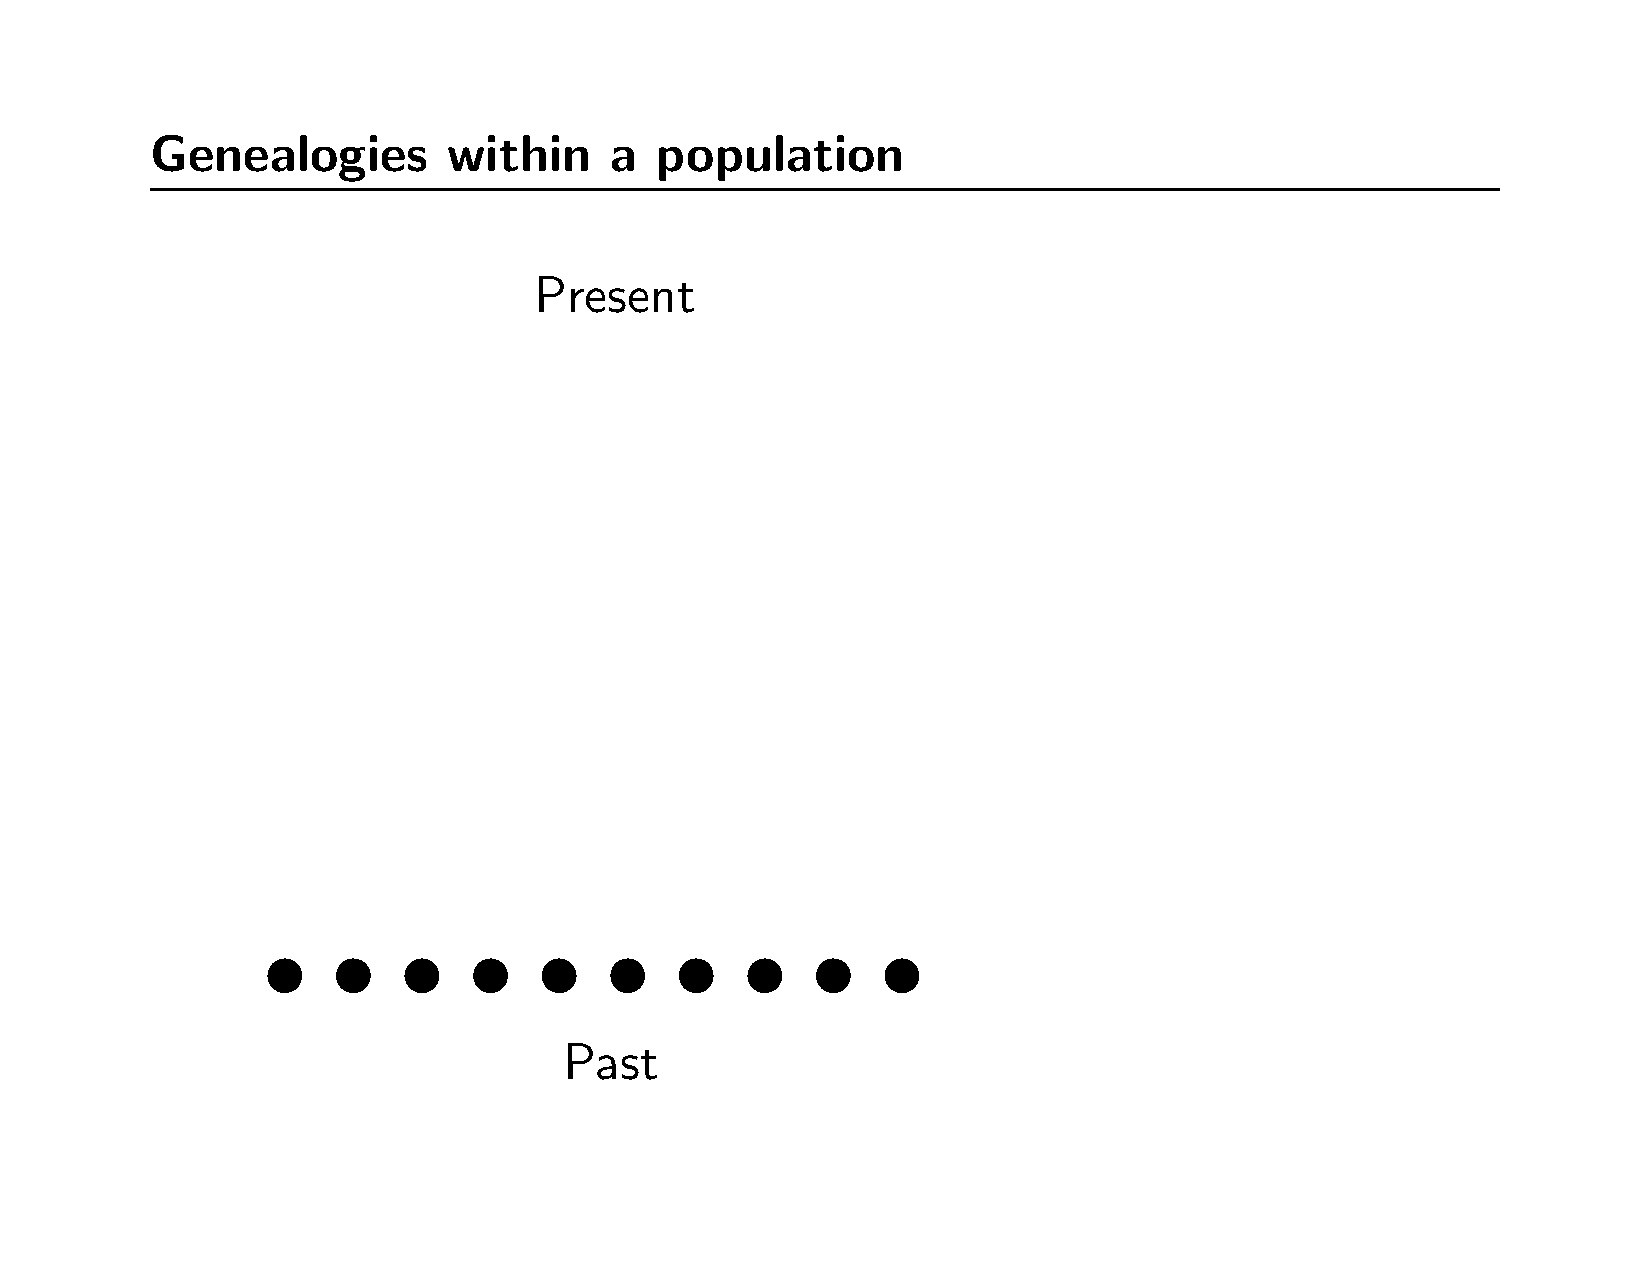
\includegraphics[page=1,height=\textheight]{../images/wright-fisher-mth.pdf}}
\frame[plain]{\includegraphics[page=2,height=\textheight]{../images/wright-fisher-mth.pdf}}
\frame[plain]{\includegraphics[page=3,height=\textheight]{../images/wright-fisher-mth.pdf}}
\frame[plain]{\includegraphics[page=4,height=\textheight]{../images/wright-fisher-mth.pdf}}
\frame[plain]{\includegraphics[page=5,height=\textheight]{../images/wright-fisher-mth.pdf}}
\frame[plain]{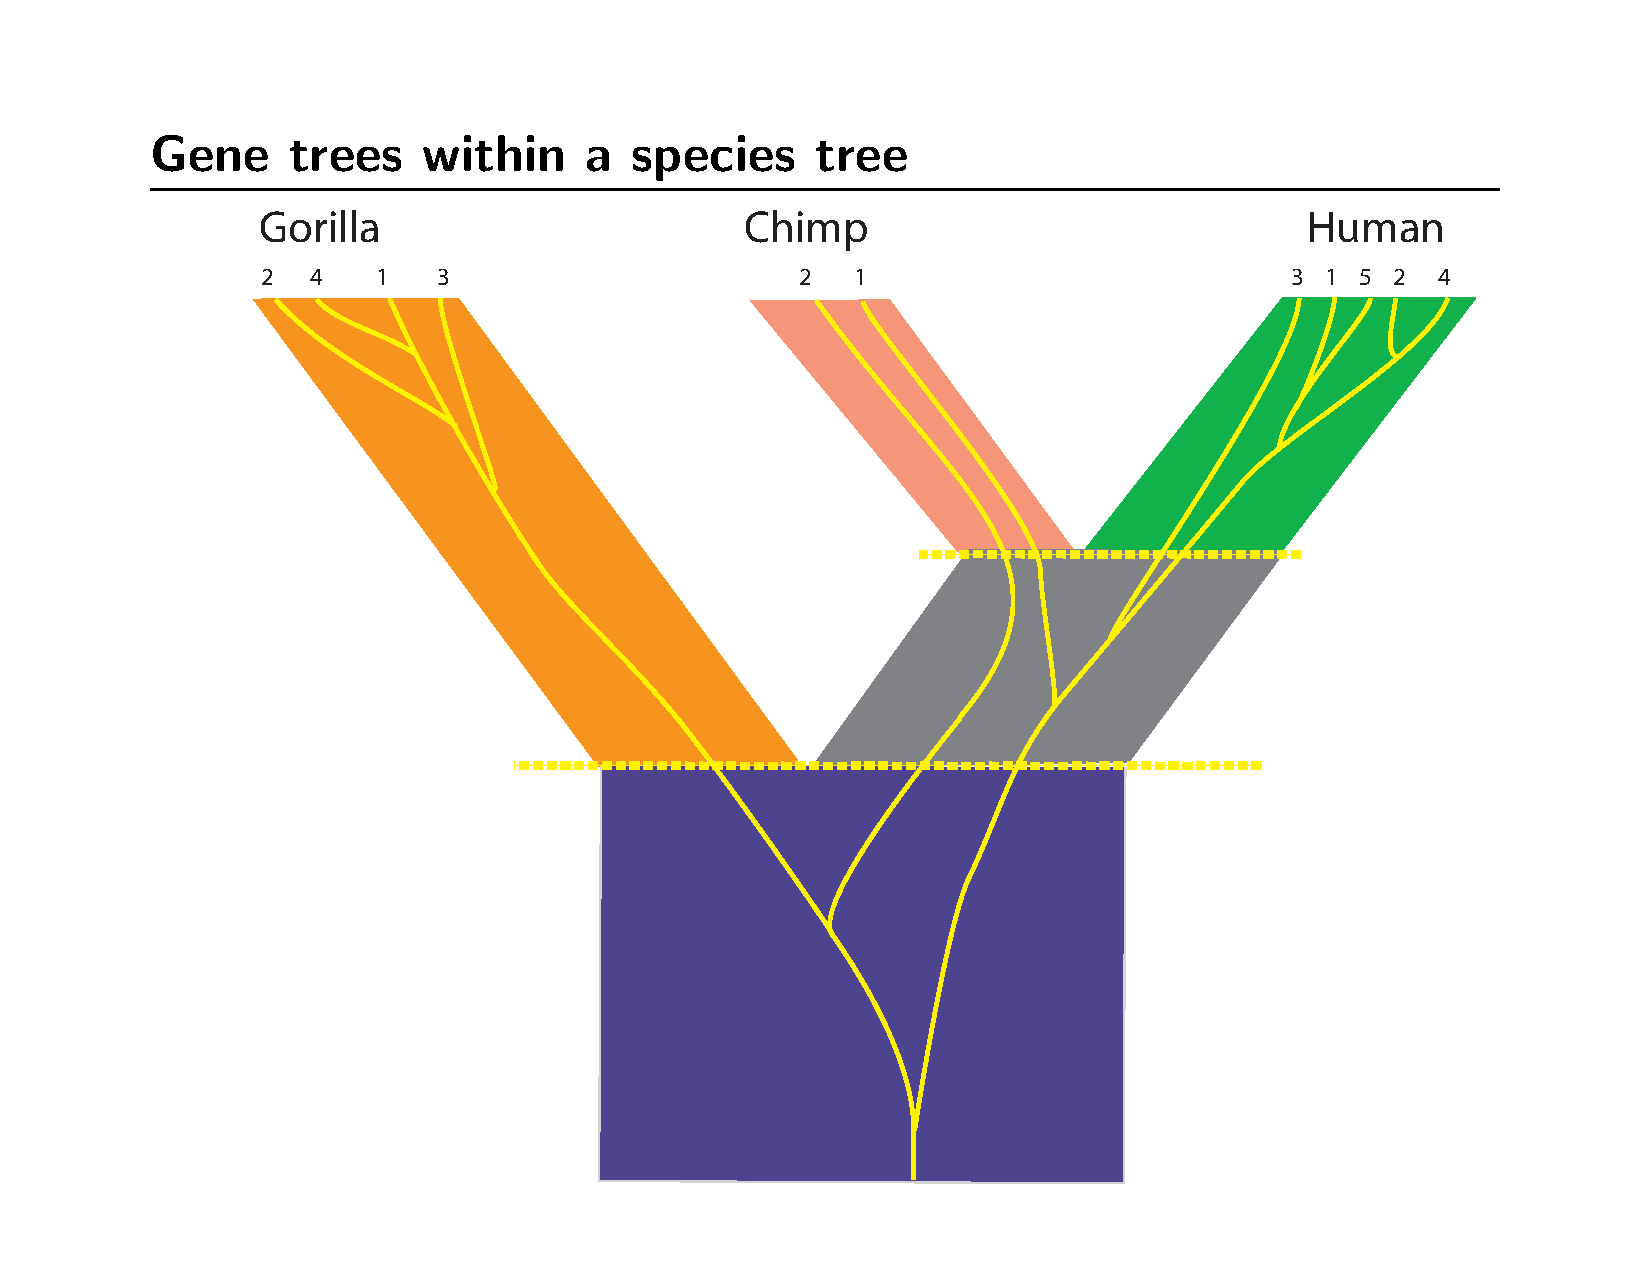
\includegraphics[page=1,height=\textheight]{../images/species-tree-slide-mth.pdf}}

\begin{frame}
    \frametitle{Phylogeography---West Nile Virus}
    \begin{figure}
        \begin{center}
        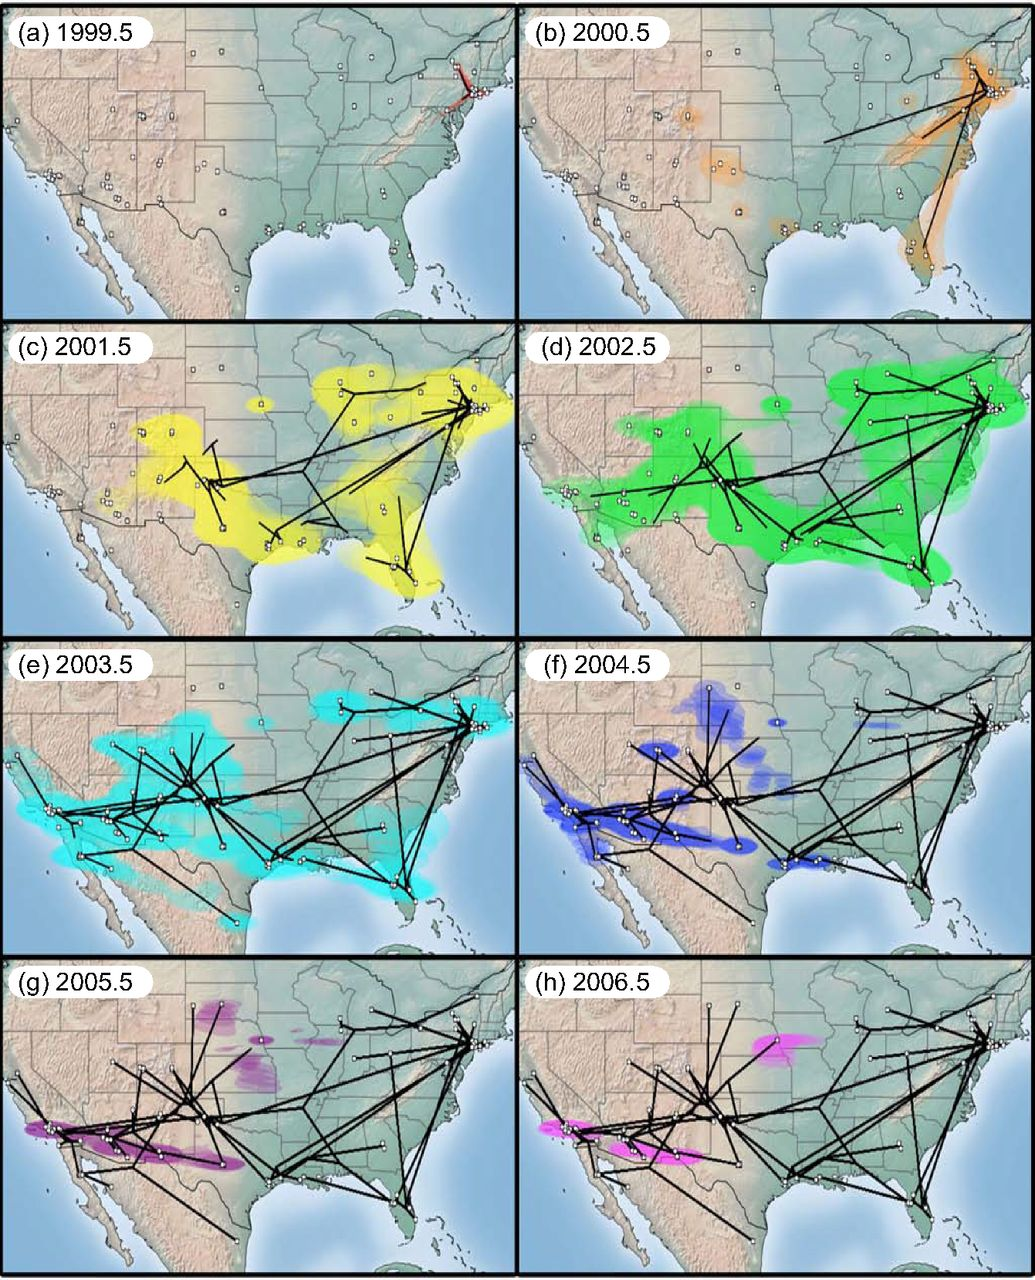
\includegraphics[width=0.5\textwidth]{../images/pybus-fig2.jpg}
        \caption{\tiny Pybus et al.\ 2012.}
        \end{center}
    \end{figure}
\end{frame}

\begin{frame}
    \frametitle{Phylogeography---West Nile Virus}
    \href{http://www.pnas.org/content/suppl/2012/08/23/1206598109.DCSupplemental/sm01.mp4}{video link}
\end{frame}

% Phylogeography
    % DNA data allowed for constructing trees of individual organisms (or gene copies) within and among species
    % gene trees
    % gene copies haplotypes
    % lineage sorting
    % coalescence
    % reciprocal monophyly
    % haplotype networks
    % gene trees within species trees (div times and incongruence)
    % book highlights these as problems, but we now have models of gene trees within species trees
        % "problems" can be a benefit for estimating historical demography and geography

% ecol niche modeling.
    % means of indirectly estimating demographic changes/ distributional shifts



\end{document}

